\documentclass[a4paper,fleqn]{cas-dc}

\usepackage[authoryear,longnamesfirst]{natbib}
\usepackage[T1]{fontenc}
\usepackage[utf8]{inputenc}
\usepackage{microtype}
\usepackage{graphicx}
\usepackage{amsmath,amssymb}
\usepackage{booktabs}
\usepackage{tabularx,array}
\usepackage{xurl}
\usepackage{xcolor}
\usepackage[most]{tcolorbox}
\usepackage{float}
\usepackage{orcidlink}
\usetikzlibrary{positioning}
\setlength{\emergencystretch}{3em}

% Journal-style visual language inspired by current JSS production.
\definecolor{JSSNavy}{HTML}{17324D}
\definecolor{JSSBlue}{HTML}{2F6FA3}
\definecolor{JSSTeal}{HTML}{168AA3}
\definecolor{JSSGray}{HTML}{F0F1F2}
\definecolor{JSSGrayText}{HTML}{4F5D68}
\definecolor{JSSBorder}{HTML}{222222}
\AtBeginDocument{\hypersetup{colorlinks=true,citecolor=JSSTeal,linkcolor=JSSTeal,urlcolor=JSSTeal}}

\tcbset{
  rqbox/.style={enhanced,breakable,colback=JSSGray,colframe=JSSGray,
    boxrule=0pt,leftrule=2.3pt,left=7pt,right=6pt,top=5pt,bottom=5pt,
    sharp corners,fontupper=\small},
  synthesisbox/.style={enhanced,breakable,colback=JSSGray,colframe=JSSBorder,
    boxrule=.7pt,arc=2.2mm,left=8pt,right=8pt,top=7pt,bottom=7pt,
    fontupper=\small},
  answerbox/.style={enhanced,breakable,colback=JSSGray,colframe=JSSTeal,
    boxrule=.55pt,leftrule=2.4pt,arc=1.4mm,left=7pt,right=7pt,top=5pt,bottom=5pt,
    fontupper=\small}
}
\newcommand{\rqicon}{\tikz[baseline=-0.55ex]\node[circle,fill=black,inner sep=1.2pt,text=white,font=\scriptsize\bfseries]{?};}
\newcommand{\RQ}[2]{%
  \begin{tcolorbox}[rqbox]
  \textbf{\rqicon\; #1---}\emph{#2}
  \end{tcolorbox}}


\begin{document}
\let\WriteBookmarks\relax
\def\floatpagepagefraction{1}
\def\textpagefraction{.001}

\shorttitle{What Breaks When Scientific Software Ages?}
\shortauthors{Bouarifi et al.}

\title[mode=title]{What Breaks When Scientific Software Ages? An Empirical Study of Long-Term Reproducibility, Repairability, and Fidelity}

% Walid BOUARIFI is the sole corresponding author.
\author[1]{Walid BOUARIFI}[orcid=0009-0000-6655-5031]
\cormark[1]
\ead{w.bouarifi@uca.ma}

\author[1]{Mouad BANA}
\ead{mouadbana51@gmail.com}

\author[1]{Soufiane KHIRI}
\ead{s.khiri@uca.ac.ma}

\affiliation[1]{organization={Laboratory in Intelligent and Sustainable Technologies (LaRTID), National School of Applied Sciences of Marrakech, Cadi Ayyad University},
                city={Marrakech},
                country={Morocco}}

\cortext[1]{Corresponding author: Walid BOUARIFI}

\begin{abstract}
\textbf{Context.} Scientific software can remain publicly available while the environments, toolchains, hardware assumptions, and validation evidence needed to reproduce its results decay. \textbf{Objective.} We investigate where long-term reproducibility degrades, why it degrades, and whether bounded repair restores downstream scientific capabilities. \textbf{Method.} We conduct an evidence-aware multiple-case study of ten heterogeneous artifacts spanning Python/PyTorch, Java, C, C++, CUDA, and R, representing approximately 180 person-hours of reconstruction, execution, evidence recovery, and analysis. Each case is classified across availability, installability, buildability, executability, scientific-result fidelity, and performance fidelity; external hardware/infrastructure eligibility, repair depth, failure mechanisms, and claim-level provenance are tracked separately. \textbf{Results.} All ten artifacts remained available, but downstream evidence thinned markedly. Only one retained case reached full execution out of the box. Three initially failing cases were recovered to full execution after bounded dependency/toolchain or build/workflow intervention, while three remained partially executable. Two cases could not be execution-tested because required external hardware/infrastructure was unavailable, and one historical execution remained evidentially unknown. Scientific fidelity was fully established in two of four eligible cases and partial in two; performance evidence was interpretable but not fully comparable in the two eligible cases. \textbf{Conclusions.} In this purposive corpus, reproducibility was better characterized by capability-specific degradation, repairability, and evidentiary support than by a binary artifact label. Long-term artifact evaluation should therefore separate execution, scientific fidelity, performance fidelity, external eligibility, and provenance.
\end{abstract}

\begin{highlights}
\item Ten scientific software artifacts were deeply reconstructed in approximately 180 person-hours.
\item Availability did not imply execution or scientific-result fidelity.
\item Bounded repairs recovered several artifacts without scientific-code changes.
\item Scientific-result and performance fidelity degraded independently.
\item Claim-level provenance exposes uncertainty hidden by binary labels.
\end{highlights}

\begin{keywords}
scientific software \sep computational reproducibility \sep software evolution \sep software artifacts \sep empirical software engineering \sep reproducibility debt
\end{keywords}

\maketitle

\section{Introduction}

Computational reproducibility is commonly understood as obtaining consistent results from the same data, computational steps, methods, code, and analysis conditions \citep{nasem2019reproducibility}. In practice, however, a published result depends on more than the continued availability of source code. Package repositories change, APIs disappear, compilers and runtimes evolve, paths and datasets become detached from workflows, and accelerators or virtualization layers may no longer be available. An artifact can therefore remain downloadable while losing one or more capabilities required to recover its scientific result.

Current artifact-evaluation practice usefully distinguishes availability, functionality, reusability, and reproduced results \citep{acm2020badging}. Reproducible-computing guidance likewise emphasizes recording commands, intermediate results, versions, and execution environments \citep{sandve2013ten}. Containers and environment-reconstruction tools improve this record, but they do not by themselves preserve external hardware, repositories, drivers, data orchestration, or performance behavior \citep{boettiger2015docker,chan2023rang}. Long-term evaluation consequently needs to identify \emph{where} the reproduction chain stops and \emph{what} was required to extend it.

We report an evidence-aware multiple-case study of ten published artifacts (PS001--PS010) spanning Python/PyTorch, Java, C, C++, CUDA, and R. The corpus was selected purposively for maximum variation in scientific domain, ecosystem, preservation mechanism, expected output, and likely aging mechanism. We operationalize reproducibility not as a binary artifact property but as a \textbf{repair-aware, evidence-bounded capability profile}: artifact availability (A), installability (I), buildability (B), executability (E), numerical or scientific fidelity (N), and performance fidelity (P). Hardware or infrastructure satisfiability (H) is recorded separately as an external eligibility condition. This representation prevents a missing GPU, an unavailable historical trace, partial scientific output, and a failed correctness check from being collapsed into the same label.

The central gap is therefore not whether scientific artifacts decay---that is already established---but what happens \emph{between} artifact availability and scientific reproduction when an aged artifact is actually reconstructed: where the capability chain stops, whether the stopping point is externally imposed or software-internal, how much bounded repair restores progress, and whether recovered execution preserves scientific and performance fidelity. This leads to a simple organizing proposition:
\[
\text{artifact survival}\not\Rightarrow\text{capability survival},
\]
with execution, scientific fidelity, and performance fidelity treated as distinct endpoints.

The study required approximately \textbf{180 person-hours} across artifact recovery, environment reconstruction, execution, intervention logging, evidence normalization, and cross-case analysis. All quantitative statements are derived from the retained case evidence through a reproducible analysis pipeline. \protect\path{N/A} and \texttt{UNKNOWN} cells remain visible and are excluded from dimension-specific denominators.

The contributions are threefold:
\begin{enumerate}
\item a \textbf{diagnostic capability model} that separates A/I/B/E/N/P outcomes from external hardware/infrastructure eligibility H;
\item a \textbf{repair-aware empirical study} of ten maximally varied aged artifacts that separates initial outcome, bounded intervention depth, recovery status, and non-exclusive failure/drift mechanisms; and
\item an \textbf{evidence-bounded fidelity analysis} with claim-level provenance, explicit \protect\path{N/A}/\texttt{UNKNOWN} handling, and an operational separation of successful execution, scientific-result fidelity, and performance fidelity (\(E\neq N\neq P\)).
\end{enumerate}

Together, these contributions support a diagnostic rather than prevalence-oriented study. Larger studies establish broader baselines; our design trades statistical breadth for per-case resolution needed to inspect install/build/run transitions, bounded repairs, external eligibility, numerical evidence, performance evidence, and provenance in the same artifact. Accordingly, the claims remain analytical and case-bounded: the corpus can demonstrate that capabilities degrade independently and expose mechanisms by which this occurs, but it does not estimate population-wide failure rates.

\section{Background and Related Work}

\subsection{Computational reproducibility and research artifacts}

We use \emph{computational reproducibility} for consistent results obtained with the original data and computational procedure, distinguishing it from replication with newly collected data \citep{nasem2019reproducibility}. This definition makes code and data necessary inputs but does not imply that their availability is sufficient. ACM artifact review similarly separates an artifact being available from it being functional, reusable, or capable of reproducing reported results \citep{acm2020badging}. Our A/I/B/E/N/P model extends this separation for retrospective diagnosis: it decomposes functionality into successive capabilities and treats hardware and infrastructure as an external eligibility condition.

\subsection{Software aging, environment evolution, and preservation}

Established guidance recommends retaining exact inputs, commands, seeds, intermediate results, software versions, and executable descriptions of analyses \citep{sandve2013ten}. Containerization can package much of the operating environment and improve portability \citep{boettiger2015docker}. Yet a container still depends on image availability, host compatibility, drivers, and suitable hardware. Environment reconstruction is particularly difficult in package ecosystems whose repositories and dependency graphs evolve. The \texttt{rang} work, for example, treats historical R-environment recovery as a distinct reconstruction problem spanning the operating system, system libraries, R version, and package versions \citep{chan2023rang}.

Longitudinal evidence confirms that artifacts degrade even after publication. Guilloteau et al. examined artifacts from leading parallel and distributed systems conferences and found systematic decay in availability and executability as time since publication increased \citep{guilloteau2024longevity}. This aging perspective motivates our retrospective framing. We revisit artifacts after their original publication environment has evolved and record the intervention required to restore each capability.

Recent work also addresses the reconstruction mechanisms themselves. R4R dynamically traces R and system dependencies to construct self-contained execution environments \citep{donatbouillud2025r4r}, while Sirvent et al. synthesize reproducibility challenges specific to HPC and distributed environments, including nondeterminism, performance, committees, and workflows \citep{sirvent2025hpc}. Together, these studies motivate the environment and infrastructure dimensions of our analysis.

These approaches are mainly prospective preservation mechanisms or reconstruction techniques. Our study asks a complementary retrospective question: when heterogeneous published artifacts are revisited, which capability remains supported by evidence, which prerequisite is unsatisfied, and what repair separates initial failure from the final state?

Environment variation is likewise not a new concern. Acher et al. frame reproducibility as a deep-variability problem spanning interacting layers such as languages, libraries, compilers, virtual machines, operating systems, and environment variables \citep{acher2024variability}. Their vision motivates systematic exploration of a validity envelope. The present study is narrower: it records the configurations actually evidenced in a retrospective recovery and does not estimate isolated effects for each layer.

\subsection{Testing scientific software and result fidelity}

Testing scientific software is itself an established research area. Kanewala and Bieman's systematic review identified 62 relevant studies and organized the challenges around properties of scientific computation---especially the difficulty of determining correct outputs---and differences between scientific and conventional software-development practice \citep{kanewala2014testing}. More recently, Eisty, Kanewala, and Carver surveyed research-software developers and found wide variation in testing practice, with test-case design, test quality, and output correctness among the principal challenges \citep{eisty2025testing}. This literature makes clear that the testing problem, including the oracle problem, is already well established.

Metamorphic testing is one established response when exact expected outputs are unavailable: instead of requiring one known result, it evaluates relations that should hold across transformed inputs or executions. It has already been applied explicitly to scientific software \citep{ding2016metamorphic}. Metamorphic relations are therefore relevant to future scientific-result contracts, although they are outside the empirical scope of the present study.

Scientific regression testing is also established practice rather than terminology introduced here. The CIAO release process combines unit, integration-oriented, regression, and package tests, including repeated testing across supported platforms to maintain scientifically valid results \citep{lee2011ciao}. Our focus is instead retrospective: we ask what scientific evidence remains supportable after heterogeneous artifacts and their execution environments have aged.

\subsection{Reproducibility debt, readiness, and research gap}

Hassan et al. conceptualize \emph{Reproducibility Debt} (RpD) as the accumulation of technical and workflow impediments that make scientific results progressively harder to reproduce \citep{hassan2025debt}. Their JSS systematic literature review screened 2,198 studies and retained 214 primary studies, from which it derived 37 causes of RpD, 63 effects grouped into seven categories, 29 prevention strategies, and 39 specialized tools or frameworks. This breadth is directly relevant here: it establishes that reproducibility degradation is not reducible to one dependency or packaging problem, but spans interacting software, workflow, environment, documentation, and infrastructure concerns. Our study complements that literature-level taxonomy with retrospective artifact-level evidence. Our analysis instead follows where an aged artifact stops along A/I/B/E/N/P, record the evidenced mechanism, quantify the bounded intervention required for recovery, and then ask whether recovered execution still supports scientific-result and performance fidelity. Repair level is therefore kept distinct from both failure mechanism and final capability outcome.

ReproScore offers another relevant distinction between static reproducibility readiness and execution-based outcome. Its 2026 preprint evaluates 423 GitHub repositories and reports that repository readiness indicators do not by themselves predict binary execution success \citep{samuel2026reproscore}. Although currently available as a preprint, its readiness/outcome separation reinforces the need to avoid inferring execution from repository contents alone. Our model further decomposes observed outcomes into execution, numerical/scientific fidelity, and performance fidelity instead of combining them into a single score.

The closest large-scale manual comparison is the ICSE 2026 study of Al Muttakin et al., which selected 100 replication packages from ICSE papers published between 2015 and 2024 and devoted approximately 650 person-hours to execution and reproduction attempts \citep{muttakin2026openscience}. Only 40 of the 100 artifacts were fully executable. Among those 40 executable artifacts, 14 reproduced the original results (35\% of the executable subset; 14\% of the full evaluated corpus). The distinction matters here: even a substantially larger manual corpus experienced a steep reduction in the number of cases eligible for downstream reproducibility assessment. The same study reports that only 32.5\% of the executable artifacts ran without modification and that 82.5\% of the executable subset required moderate-to-high effort, while identifying 13 challenge types spanning environmental, documentation, and structural issues. These results provide a strong prevalence baseline and independently reinforce the need to distinguish availability, executability, repair effort, and result reproduction instead of collapsing them into one binary label.

Against that large-scale baseline, our ten-case corpus serves a different purpose: it is a deliberately deep, heterogeneous diagnostic corpus. The unit of contribution is the reconstructed capability profile of each case: availability, installability, buildability, executability, numerical/scientific fidelity, performance fidelity, external eligibility, bounded repair, and claim-level provenance. This design trades statistical breadth for diagnostic resolution. It also prevents a missing GPU (PS002) or an infrastructure constraint (PS007) from entering the executability denominator as a software failure, and prevents partially successful executions such as PS005 and PS010 from being treated identically to a failed one.

CompRep provides a complementary curated benchmark for computational-reproducibility tools. Its authors collected 38 experiments and report that 18 could be executed with at least one evaluated tool, while emphasizing missing artifacts, version incompatibilities, and incomplete environment documentation \citep{costa2025comprep}. This benchmark is broader as a reusable tool-evaluation dataset; our closed corpus instead emphasizes longitudinal aging, bounded repair, downstream N/P status, and claim-level evidence provenance.

Finally, reproducibility literature already considers how experimental choices and uncontrolled variation can affect inferred conclusions. Gundersen et al. organize such sources for machine learning in a framework running from experimental design to conclusions \citep{gundersen2022sources}. We therefore do not claim that conclusion reproducibility is a new concept. More importantly, the current cases do not uniformly encode publication claims as executable predicates, so conclusion stability remains outside our measured outcomes.

\paragraph{Positioning of this study.}

Figure~\ref{fig:1} organizes the four research streams that most directly delimit our contribution. They establish artifact availability, environment preservation, scientific-output testing, and execution assessment as prior work. The present study connects these streams through a retrospective capability chain at artifact level.

\begin{figure*}[t]
\centering
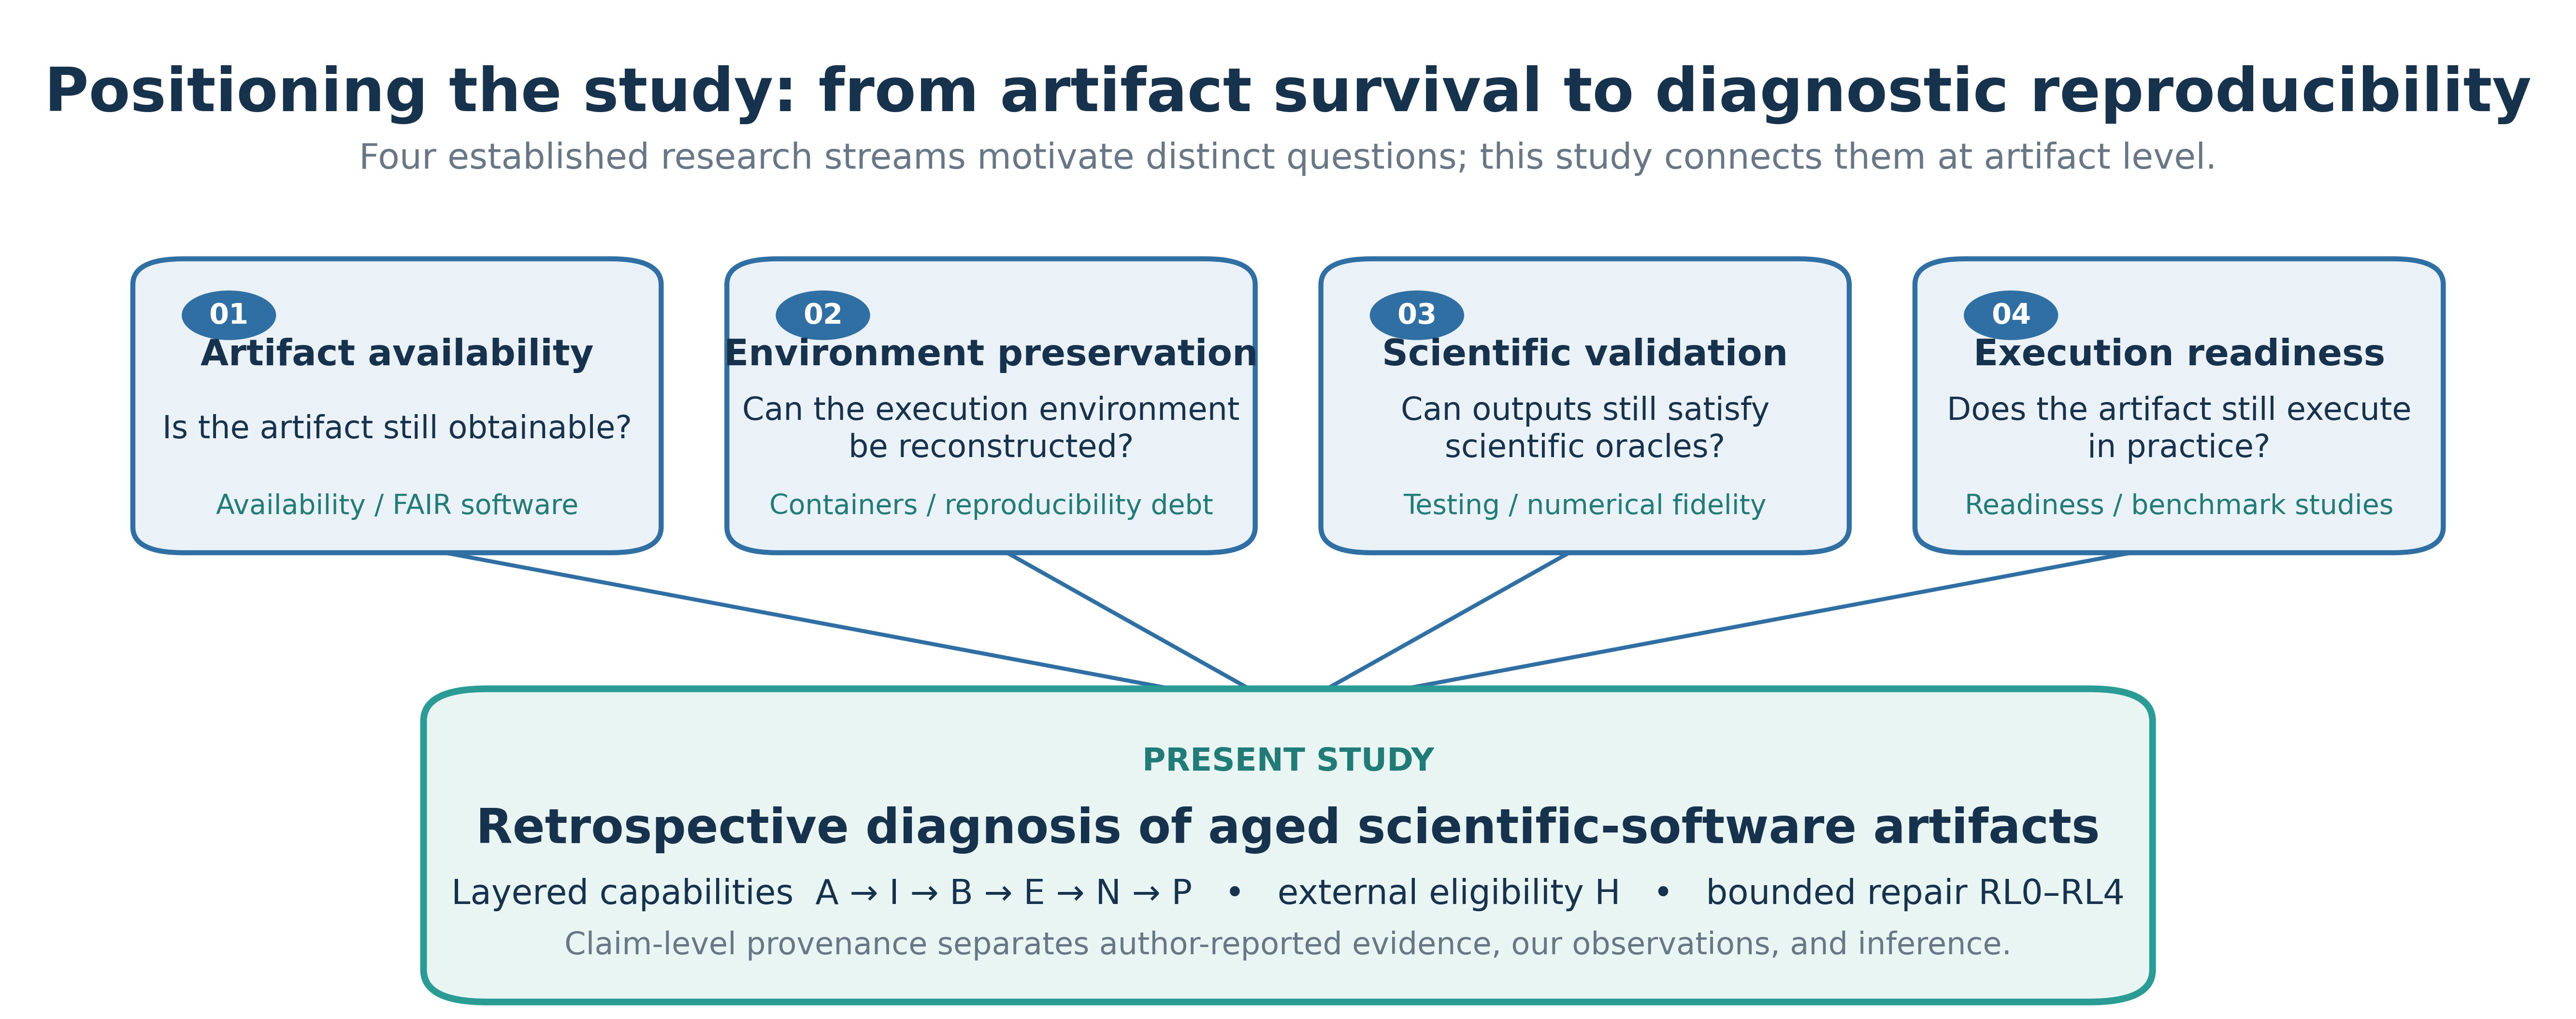
\includegraphics[width=0.92\textwidth]{Figure_01.png}
\caption{Positioning of the present study relative to artifact evaluation, environment preservation, scientific-software testing, and execution-oriented reproducibility research. The figure is a conceptual literature map rather than a quantitative result.}
\label{fig:1}
\end{figure*}

\begin{tcolorbox}[synthesisbox]
Prior studies establish the persistence problem at complementary levels: artifact availability, environment reconstruction, execution readiness, and scientific validation. The gap addressed here is narrower and diagnostic: once an aged artifact is obtainable, we trace which capability remains supported, which mechanism interrupts progression, how much bounded repair is needed, and whether recovered execution also preserves scientific and performance fidelity. This positioning complements rather than replaces the larger prevalence studies cited above.
\end{tcolorbox}

The conceptual map in Fig.~\ref{fig:1} identifies the neighboring research streams; Table~\ref{tab:1} makes the boundary operational. It compares the unit of analysis and endpoint of each stream with the dimensions retained here, so that the contribution is read as an extension in diagnostic resolution rather than as a claim that availability, preservation, testing, or execution assessment are themselves new. In particular, the RpD synthesis of Hassan et al. supplies a broad taxonomy of accumulated causes and effects, whereas our empirical protocol traces how such impediments materialize within individual aged artifacts and whether bounded repair restores downstream capability.

\begin{table*}[t]
\centering
\caption{Analytical distinction between nearest research streams and the present study. "Not evaluated" identifies a scope boundary rather than a weakness attributed to the cited work.}
\label{tab:1}
\footnotesize
\setlength{\tabcolsep}{3pt}
\begin{tabularx}{\textwidth}{@{}>{\raggedright\arraybackslash}X>{\raggedright\arraybackslash}X>{\raggedright\arraybackslash}X>{\raggedright\arraybackslash}X@{}}
\toprule
Research stream & Primary unit or endpoint & What it establishes & Relation to this study \\
\midrule
Artifact evaluation and availability & Published artifact & Availability, functionality, reuse, or reproduced-result categories & Supplies upstream vocabulary; our analysis decomposes post-availability capability \\
Environment preservation and reproducibility debt & Workflow or environment & Reconstruction mechanisms and accumulated impediments; Hassan et al. synthesize 37 causes, 63 effects, 29 prevention strategies, and 39 tools/frameworks & Provides the broad RpD problem space; our RL and mechanism fields operationalize observed case-level interruption and recovery \\
Scientific-software and metamorphic testing & Program properties and test oracles & Ways to detect incorrect or inconsistent scientific behavior & Establishes prior art; no testing framework is evaluated here \\
Readiness, execution, and benchmark datasets & Repository or executable experiment & Static readiness, execution outcome, or tool-comparison benchmark & Nearest execution-level comparison; our model separately retains N and P \\
Al Muttakin et al. (ICSE 2026) & 100 SE replication packages & Prevalence of executability, effort categories, and 13 challenge types & Establishes a prevalence baseline; our model adds N/P separation, H eligibility, and claim-level provenance \\
Guilloteau et al. (ACM REP 2024) & HPC/parallel artifacts, longitudinal & Availability and executability decay after publication & Motivates the aging framing; our study adds per-case diagnostic depth with repair tracing \\
Present multiple-case study & Aged paper-linked artifact & A/I/B/E/N/P state, H eligibility, repair depth, and claim provenance & Retrospective diagnostic synthesis over PS001--PS010; not a prevalence or causal study \\
\bottomrule
\end{tabularx}
\end{table*}

Empirical work on software artifacts has documented both increasing availability and continuing weaknesses in publication, maintenance, documentation, and persistence. Heumüller et al. examined 789 ICSE papers from 2007--2017 and distinguished papers that claim software artifacts from artifacts that remain publicly obtainable \citep{heumueller2020artifacts}. Liu et al. later analyzed 1,487 artifacts associated with 2,196 papers from four software-engineering venues published between 2017 and 2022, focusing on availability, maintenance, popularity, and quality \citep{liu2024artifacttrends}. These studies establish that artifact publication and continued availability are substantive empirical concerns.

Our question begins after availability has been assessed. We examine whether an obtainable artifact can still traverse dependency resolution, build, execution, scientific validation, and performance comparison, and we record the intervention required to move between those layers. The focus is diagnostic and retrospective; it is not a prevalence study of artifact-sharing practice.

Existing large-scale studies establish prevalence baselines for executability and binary result reproduction \citep{muttakin2026openscience,costa2025comprep,samuel2026reproscore}, and longitudinal studies document availability decay \citep{guilloteau2024longevity,heumueller2020artifacts}. What is comparatively less explicit in the nearest execution-oriented studies is the combined diagnostic decomposition of post-repair outcomes used here: specifically, whether an artifact that becomes executable after bounded intervention also satisfies its artifact-native numerical or scientific criteria (N), and whether numerical correctness implies performance preservation (P). The H eligibility condition additionally keeps hardware or infrastructure unsatisfiability outside the software-failure numerator in our protocol; this is a study-design distinction rather than a claim that prior work ignored hardware requirements altogether. The present corpus provides case-level evidence for this layered distinction, with explicit \texttt{PARTIAL}, \protect\path{N/A}, and \texttt{UNKNOWN} states and denominator-aware reporting. Together, these comparisons locate the contribution at the intersection of post-publication reconstruction, bounded repair, and downstream fidelity assessment.

\section{Study Design}

\subsection{Research questions}

We organize the study around four research questions that separate observable capability, failure mechanism, intervention depth, and downstream fidelity.

\RQ{RQ1}{Which reproducibility capabilities remain supportable when published scientific-software artifacts are revisited in contemporary environments?}
RQ1 asks \textbf{what survives}. It establishes the evidence-supported capability profile across A/I/B/E/N/P, with H treated as an eligibility modifier rather than a software outcome.

\RQ{RQ2}{Which technical and evidentiary mechanisms interrupt or weaken those capabilities?}
RQ2 identifies the non-exclusive mechanisms observed in the retained evidence, including dependency decay, runtime sensitivity, environment coupling, hardware constraints, virtualization decay, and trace loss.

\RQ{RQ3}{To what extent can degraded artifacts recover downstream capabilities through bounded intervention without scientific-code modification?}
RQ3 asks \textbf{what can be recovered}. RL0--RL4 records intervention depth, while a separate recovery status records whether the attempted reconstruction was recovered, partial, unrecovered, or not attempted.

\RQ{RQ4}{When execution is available or recovered, to what extent are scientific-result and performance fidelity preserved?}
RQ4 separates scientific-result fidelity (N) from performance fidelity (P). This avoids treating successful execution, numerical correctness, and performance comparability as equivalent outcomes.

Containers, virtual machines, dependency specifications, and build systems are analyzed as cross-cutting preservation mechanisms within RQ2--RQ4 rather than as a separate research question.

\begin{table*}[t]
\centering
\caption{Research-question-to-evidence map. The table makes explicit which retained evidence stream supports each answer and prevents an execution observation from being silently promoted to a fidelity claim.}
\label{tab:rqmap}
\small
\setlength{\tabcolsep}{5pt}
\begin{tabularx}{\textwidth}{@{}p{0.07\textwidth}>{\raggedright\arraybackslash}p{0.24\textwidth}>{\raggedright\arraybackslash}p{0.31\textwidth}>{\raggedright\arraybackslash}X@{}}
\toprule
RQ & Analytical target & Primary retained evidence & Output used in the answer \\
\midrule
RQ1 & Long-term capability & Commands, build/run logs, environment records, A/I/B/E/N states & Layered matrix; execution outcome summary \\
RQ2 & Failure mechanisms & Raw failures, intervention records, mechanism adjudication & Non-exclusive mechanism taxonomy and counts \\
RQ3 & Repairability & Before/after logs, repair descriptions, RL0--RL4 classification plus recovery status & Recovery status and maximum repair depth \\
RQ4 & Scientific/performance fidelity & Artifact-native verification, checksums, metrics, repeated benchmarks & N/P states; PS003 uncertainty; PS008 configuration comparison \\
\bottomrule
\end{tabularx}
\end{table*}

Table~\ref{tab:rqmap} defines what evidence is allowed to answer each research question; Fig.~\ref{fig:evidencechain} then shows how that evidence is transformed without skipping provenance or decision rules. The sequence is deliberate: raw logs and outputs first acquire a claim-level source, are normalized under the fixed classification vocabulary, enter the capability matrix, and only then support an RQ-level statement. This prevents a successful command, an author-reported value, or an inferred explanation from being silently treated as equivalent forms of evidence.

\begin{figure*}[t]
\centering
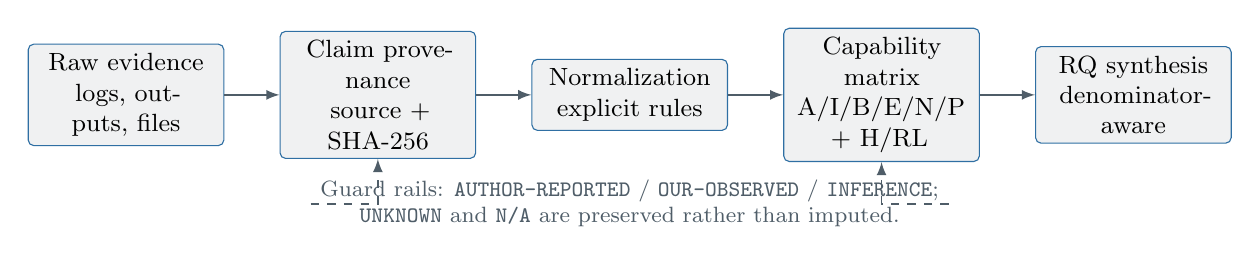
\begin{tikzpicture}[font=\small,>=latex,node distance=5mm and 7mm]
\tikzset{ev/.style={draw=JSSBlue,rounded corners=2pt,fill=JSSGray,align=center,minimum height=9mm,text width=2.25cm},
         arr/.style={->,draw=JSSGrayText,line width=.65pt}}
\node[ev] (raw) {Raw evidence\\logs, outputs, files};
\node[ev,right=of raw] (prov) {Claim provenance\\source + SHA-256};
\node[ev,right=of prov] (norm) {Normalization\\explicit rules};
\node[ev,right=of norm] (matrix) {Capability matrix\\A/I/B/E/N/P + H/RL};
\node[ev,right=of matrix] (rq) {RQ synthesis\\denominator-aware};
\draw[arr] (raw)--(prov); \draw[arr] (prov)--(norm); \draw[arr] (norm)--(matrix); \draw[arr] (matrix)--(rq);
\node[below=5mm of norm,align=center,text=JSSGrayText,font=\footnotesize] (guard) {Guard rails: \texttt{AUTHOR-REPORTED} / \texttt{OUR-OBSERVED} / \texttt{INFERENCE};\\\texttt{UNKNOWN} and \texttt{N/A} are preserved rather than imputed.};
\draw[arr,dashed] (guard.west) -| (prov.south); \draw[arr,dashed] (guard.east) -| (matrix.south);
\end{tikzpicture}
\caption{Chain of evidence used in this study. Raw retained artifacts are linked to claim provenance, normalized under explicit decision rules, propagated into the layered matrix, and only then synthesized into RQ-level statements. The diagram is methodological: it does not introduce additional experimental outcomes.}
\label{fig:evidencechain}
\end{figure*}

\subsection{Design and corpus}

The unit of analysis is a published scientific-software artifact linked to an executable experimental claim. The closed corpus contains exactly PS001--PS010. It is a purposive maximum-variation sample across languages, domains, workloads, preservation mechanisms, and expected outputs, not a random sample. Cases were not added, removed, or substituted after analysis. The corpus size reflects a deliberate trade-off between breadth and diagnostic depth. Existing studies with 38 to 423 subjects establish broader baselines for execution, reproduction, or readiness \citep{muttakin2026openscience,costa2025comprep,samuel2026reproscore}. The present design instead retains 47 claim-level provenance records, separates hardware and infrastructure constraints from software failures, distinguishes N from P using artifact-native evidence, and records bounded interventions. Ten maximally varied cases therefore support analytical comparison of the layered proposition, not statistical representativeness or a prevalence estimate. This follows multiple-case design logic, where purposive variation and theoretical coverage guide case selection \citep{runeson2009guidelines}. Table~\ref{tab:2} summarizes the corpus.

\subsection{Layered capability model and decision rules}

For each case we classify the vector R=(A,I,B,E,N,P): artifact availability, installability or dependency resolution, buildability, executability, numerical or scientific fidelity, and performance fidelity. We refer to this as a \emph{layered capability model}: the ordering captures prerequisites for evaluation, but it is not a universal causal law and not every layer applies to every ecosystem. Hardware/infrastructure satisfiability H is recorded separately using \texttt{SAT}, \texttt{UNSAT}, or \texttt{UNKNOWN}. If H is \texttt{UNSAT}, downstream execution may be \protect\path{N/A} rather than \texttt{FAIL}.

Each A--P dimension uses exactly five states. \texttt{PASS} means the declared criterion was evaluated and fully supported by retained evidence; \texttt{PARTIAL} means a scientifically meaningful subset of the declared criterion was established but full satisfaction was not; \texttt{FAIL} means an eligible, explicitly evaluated criterion failed; \protect\path{N/A} means the dimension is inapplicable or cannot legitimately be attempted because an external prerequisite is unsatisfied; and \texttt{UNKNOWN} means the retained evidence is insufficient to classify it. \protect\path{N/A} and \texttt{UNKNOWN} are never silently converted to failures and are excluded from observed denominators.

For \textbf{numerical/scientific fidelity (N)}, \texttt{PASS} requires satisfaction of an explicit artifact-specific oracle, reference, verification condition, or declared numerical tolerance within the evaluated scope. \texttt{PARTIAL} is used only when a subset of required outputs or validation criteria is retained but equivalence to the full author-reported target is not established. \texttt{FAIL} requires an explicit applicable scientific criterion that was evaluated and violated. \texttt{UNKNOWN} is used when outputs exist but no defensible oracle or comparison basis is retained. Thus, a generated figure or metric is not automatically \texttt{N=PASS}.

For \textbf{performance fidelity (P)}, \texttt{PASS} requires a sufficiently comparable performance protocol/reference and evidence that the declared performance criterion is preserved within that scope. \texttt{PARTIAL} means performance was measured and is scientifically interpretable, but full comparability or stability is not established because of runtime sensitivity, substantial variability, or explicitly documented confounding. \texttt{FAIL} requires a comparable declared performance criterion that was evaluated and violated. \texttt{UNKNOWN} is used when timing/performance output exists but no defensible comparator or protocol supports a fidelity judgment. In this study, PS003 and PS008 therefore remain \texttt{P=PARTIAL}: both provide usable performance evidence, but neither supports a full performance-fidelity claim.

Figure~\ref{fig:2} summarizes the three analytical axes retained in the main paper: \textbf{capability outcome} (A--P), \textbf{intervention depth} (RL0--RL4), and \textbf{non-exclusive mechanism}. H is an eligibility modifier, while provenance constrains which claims can be made. These axes answer different questions: what capability was supported, how much intervention was required, and why the path was impeded or changed.

\begin{figure*}[t]
\centering
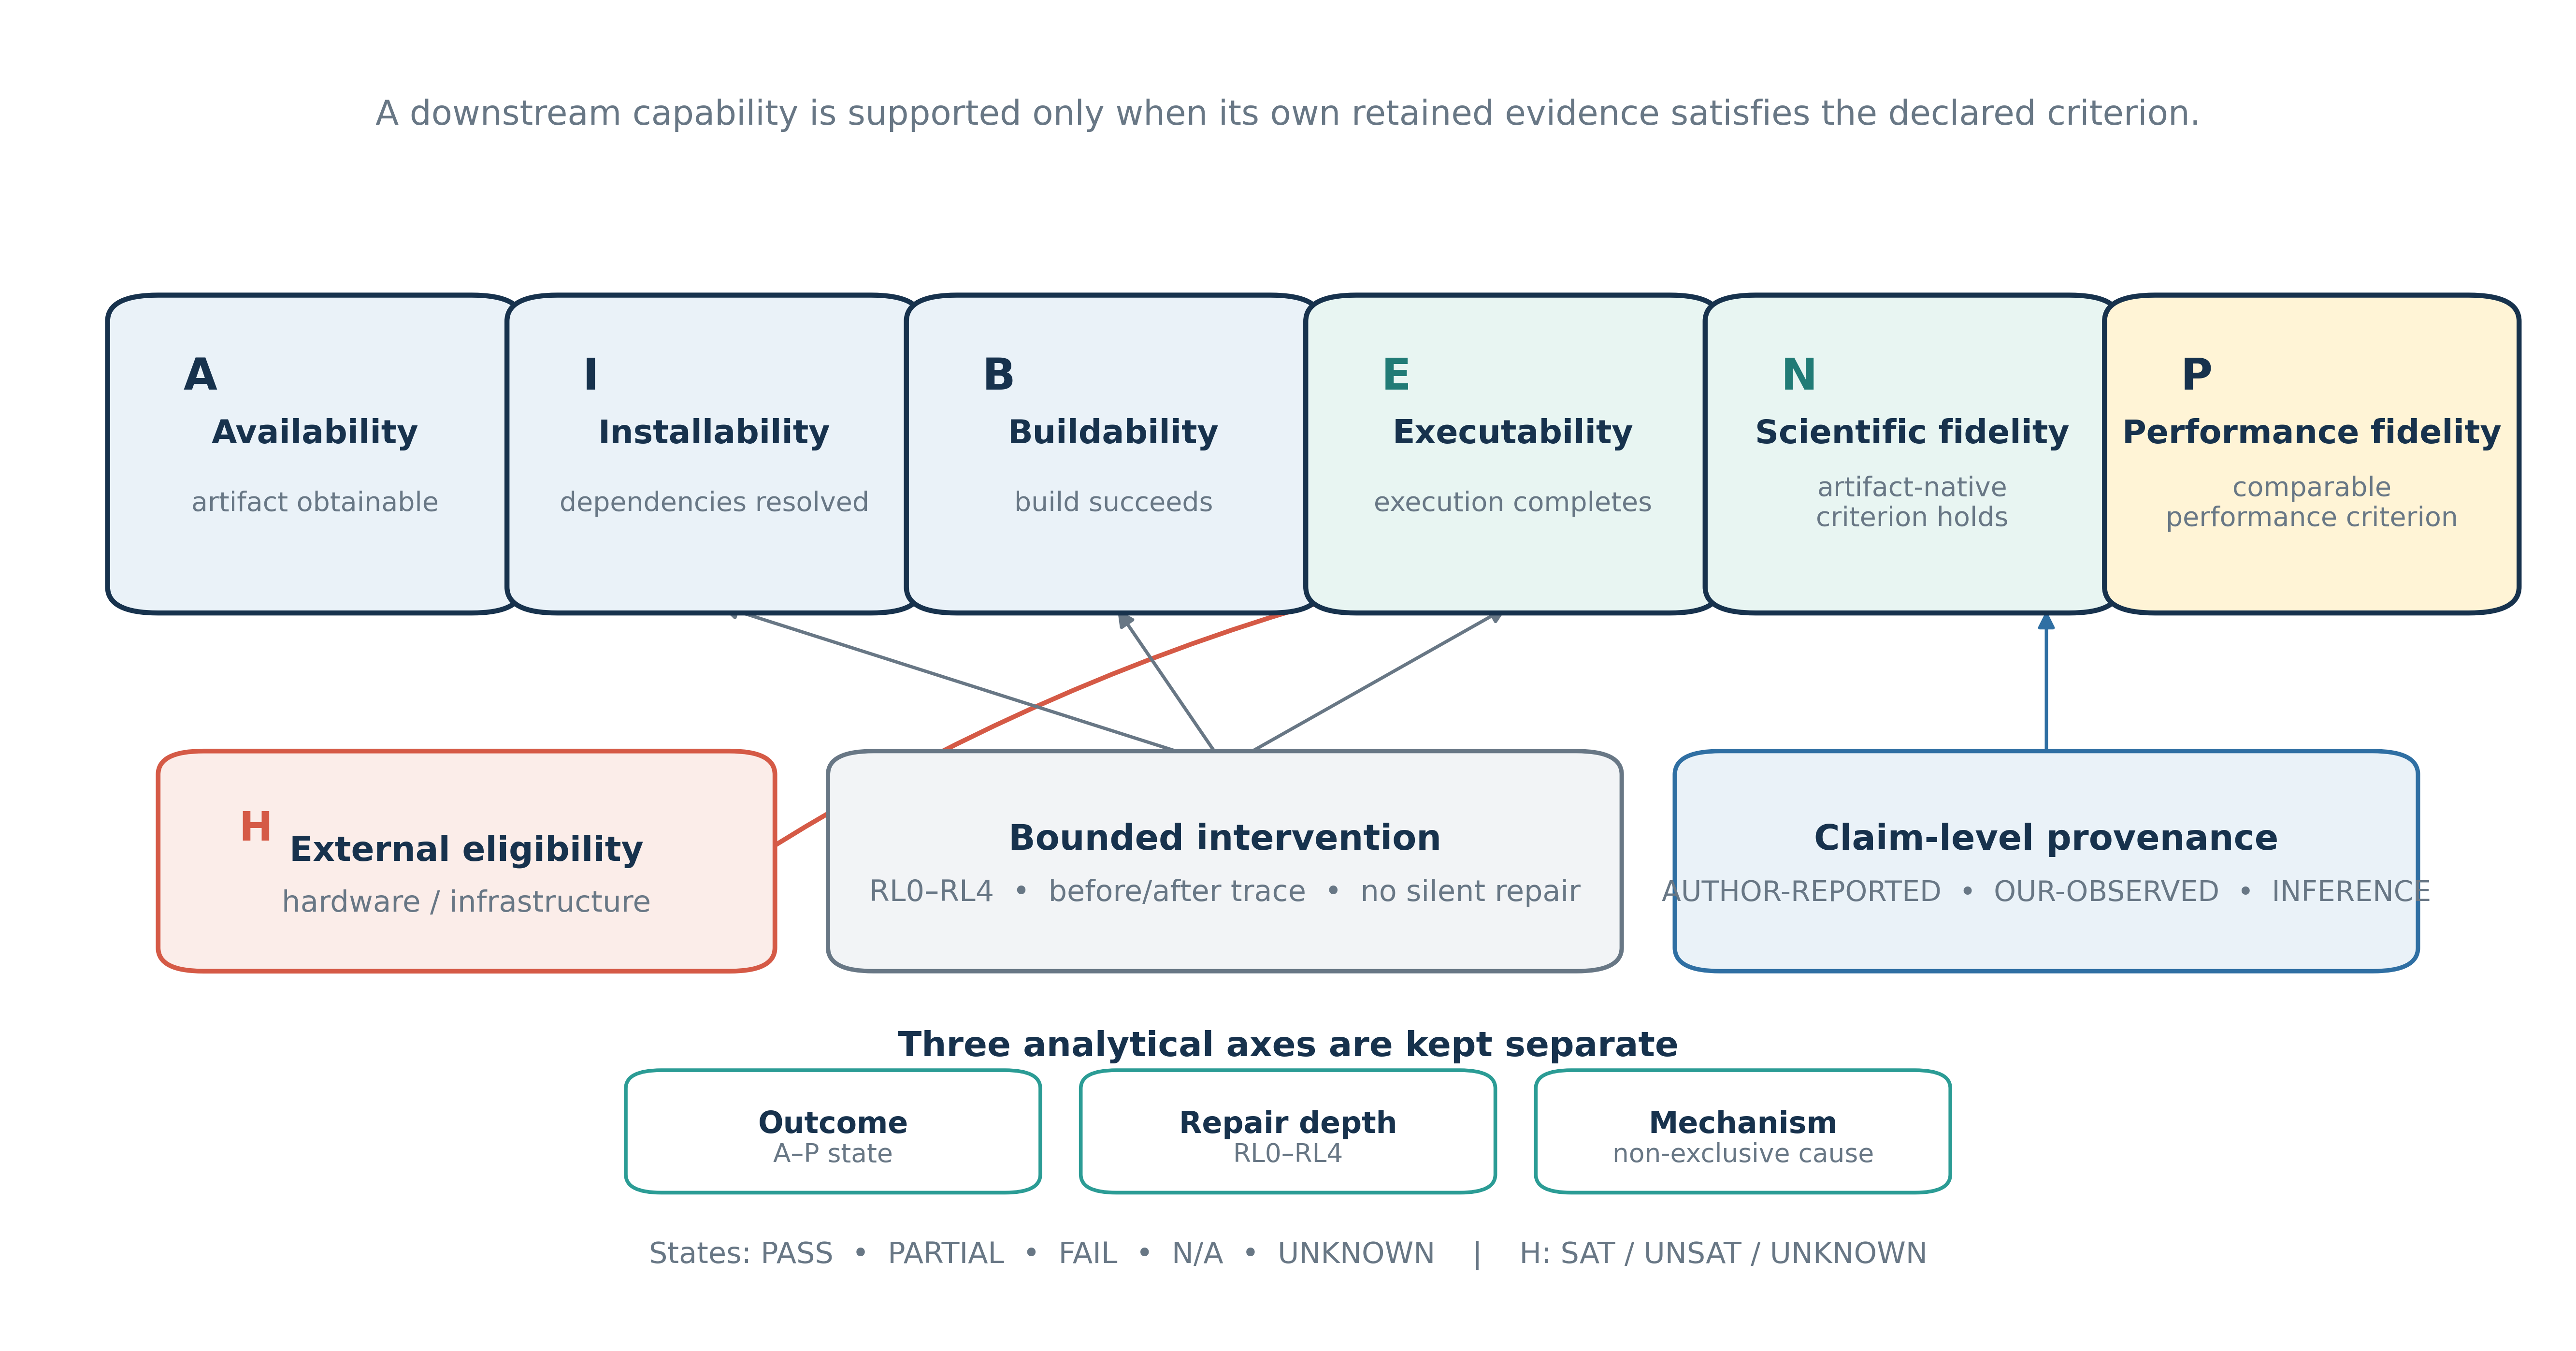
\includegraphics[width=0.92\textwidth]{Figure_02.png}
\caption{Layered reproducibility model used in the study. A, I, B, E, N, and P denote availability, installability, buildability, executability, scientific-result fidelity, and performance fidelity. Hardware/infrastructure satisfiability is an external eligibility condition; repair depth and failure mechanism are recorded separately.}
\label{fig:2}
\end{figure*}

\subsection{Experimental ladder and repairs}

The protocol proceeds, where meaningful, from E0 artifact identity and availability, through E1 contemporary out-of-the-box execution, E2 an author-provided container/VM/lockfile, E3 minimal environment or dependency repair, E4 historical runtime reconstruction, E5 numerical validation, and E6 performance validation. Later stages are attempted only when prerequisites and scientific meaning remain intact.

Intervention depth is coded RL0 (none), RL1 (environment/configuration), RL2 (dependency/toolchain), RL3 (build/packaging/path), or RL4 (scientific source modification). \textbf{Unrecovered is not an intervention level}: recovery outcome is recorded separately as \texttt{RECOVERED}, \texttt{PARTIAL}, \texttt{UNRECOVERED}, or \texttt{NOT-ATTEMPTED}. This avoids mixing repair depth with final outcome. RL1--RL3 remains distinct from RL4 because the former need not change the scientific algorithm. Interventions are logged with before/after state, rationale, and observed effect.

\subsection{Evidence and provenance}

Raw logs, outputs, environment records, and intervention histories are retained for each case in the replication package. Every manuscript claim is labeled \texttt{AUTHOR-REPORTED}, \texttt{OUR-OBSERVED}, or \texttt{INFERENCE} in the evidence registry and is linked to a supporting evidence item. Published values are never represented as reproduced measurements. Missing evidence remains \texttt{NA -- evidence unavailable}, \texttt{UNKNOWN}, or \texttt{TRACE-INCOMPLETE}; it is not reconstructed from memory. The final registry contains 47 uniquely identified claims across the ten cases.

We use \emph{trace decay} as an operational label for an evidentiary condition in which a historical experimental result is believed to have been produced, but the retained material cannot support an independent audit of the inputs, environment, commands, interventions, intermediate states, and outputs that generated it. Trace decay is orthogonal to software behavior: the artifact may remain intact, available, or re-executable while its historical evidentiary chain is broken. It is recorded as a mechanism rather than substituted for a dimension outcome. \texttt{UNKNOWN} remains the appropriate state when retained evidence cannot support a dimension classification, whereas \texttt{FAIL} requires an eligible attempted criterion that demonstrably failed. PS001 illustrates this distinction: the artifact remains available and the publication reports numerical results, but no recoverable local execution trace or environment record supports an \texttt{OUR-OBSERVED} MSE or MAE statement. Coding the historical experiment recovery status as \texttt{UNRECOVERED} and I through P as \texttt{UNKNOWN}, rather than \texttt{FAIL}, preserves the difference between \emph{could not be audited} and \emph{was observed to fail}.

A claim-to-evidence appendix is provided as supplementary material. It lists all 47 validated claims, their provenance labels, and the evidence files supporting them.

\subsubsection{Coding reliability and adjudication}

The capability states and provenance labels were assigned using a frozen codebook, explicit decision rules, and claim-linked evidence records. Disagreements encountered during evidence review were resolved by team adjudication against the retained raw material. Because no independent blinded second-coder exercise was conducted, we report no inter-rater reliability coefficient; the resulting classifications are team-adjudicated judgments.

The classification logic admits raw material to the normalized analysis only through a validated claim. An unsatisfied prerequisite yields \protect\path{N/A}; missing evidence yields \texttt{UNKNOWN} or \texttt{TRACE-INCOMPLETE}; only an eligible, evidenced criterion can receive \texttt{PASS}, \texttt{PARTIAL}, or \texttt{FAIL}. This decision structure determines the dimension-specific denominators used later. The full evidence-decision schematic is retained in the supplementary material.

\subsection{Cross-case analysis}

The normalized matrix is the single source for aggregate analysis. For dimension d, the reported denominator contains only \texttt{PASS}, \texttt{PARTIAL}, and \texttt{FAIL} cases. Percentages are therefore n(state,d)/n(eligible,d), accompanied by the denominator and counts excluded as \protect\path{N/A} or \texttt{UNKNOWN}. Failure mechanisms are non-exclusive. Repair levels and out-of-the-box outcomes are mutually exclusive case summaries.

Formally, for case set C, state s, and dimension d, the observed eligible set and state rate are

\begin{align}
C_d^{obs} &= \{i\in C : X_{i,d}\in\{\mathrm{PASS},\mathrm{PARTIAL},\mathrm{FAIL}\}\},\\
\hat p_{s,d} &= \frac{\sum_{i\in C_d^{obs}}\mathbf{1}(X_{i,d}=s)}{|C_d^{obs}|}.
\end{align}

The strict and inclusive summaries are respectively

\[
\hat p_d^{\mathrm{strict}}=\hat p_{\mathrm{PASS},d},\qquad\hat p_d^{\mathrm{inclusive}}=\hat p_{\mathrm{PASS},d}+\hat p_{\mathrm{PARTIAL},d}.
\]

For an applicable \texttt{UNKNOWN} set U\_d, classification-sensitivity bounds for the strict-pass rate are

\[
L_d=\frac{n_{PASS,d}}{|C_d^{obs}|+|U_d|},\qquad U_d=\frac{n_{PASS,d}+|U_d|}{|C_d^{obs}|+|U_d|}.
\]

PS003 performance is summarized across three independent repetitions per JDK using the mean baseline-adjusted \protect\path{ijOps/sjOps} ratio, standard deviation, coefficient of variation, and a two-sided 95\% t interval with two degrees of freedom. No cross-JDK inferential test is used. PS008 timings are descriptive comparisons of two confounded reconstructed configurations and are not interpreted as a causal version effect.

For each JDK condition j with n\_j=3 retained repetitions, the reported interval is

\[
\bar r_j\ \pm\ t_{0.975,n_j-1}\frac{s_j}{\sqrt{n_j}},
\]

where r is the baseline-adjusted \protect\path{ijOps/sjOps} ratio. Because these intervals describe three retained repetitions under each tested condition, they are not used as a population-level model of JDK effects.

Sensitivity analysis reports strict (\texttt{PASS}) and inclusive (\texttt{PASS} or \texttt{PARTIAL}) rates and worst/best bounds for applicable \texttt{UNKNOWN} cells. A transition analysis identifies adjacent decreases in the ordered chain. All matrices, summaries, tables, and figures are generated by Python from normalized inputs.

Cross-case statistics are descriptive and denominator-aware. The PS003 confidence intervals characterize three retained repetitions per JDK; they are not population estimates for all JDK configurations. PS008 remains a descriptive comparison because its configurations are confounded. Population prevalence, causal attribution, cross-case regression, and claim-stability modeling lie beyond the inference boundary of this ten-case purposive design. The full statistical-analysis map is retained in the supplementary material.

\subsection{Experimental Subjects and Setup}


\begin{table*}[t]
\centering
\caption{Closed corpus and principal reproduction target. Preservation entries describe the artifact material made available, not a guarantee of successful execution.}
\label{tab:2}
\fontsize{6}{7.2}\selectfont
\setlength{\tabcolsep}{1pt}
\begin{tabularx}{\textwidth}{@{}>{\raggedright\arraybackslash}p{0.06\textwidth}>{\raggedright\arraybackslash}p{0.22\textwidth}>{\raggedright\arraybackslash}p{0.14\textwidth}>{\raggedright\arraybackslash}p{0.20\textwidth}>{\raggedright\arraybackslash}X@{}}
\toprule
ID & Artifact & Ecosystem & Principal target & Preservation material / limiting prerequisite \\
\midrule
PS001 & DLinear / LTSF-Linear \citep{zeng2023dlinear,ltsflinearrepo} & Python/PyTorch & Forecast MSE/MAE & Repository and scripts; historical local result trace unavailable \\
PS002 & Hidet \citep{ding2023hidet} & Python/C++/CUDA & GPU compiler artifact & CUDA container; NVIDIA GPU unavailable on retained host \\
PS003 & SciJava Ops \citep{selzer2024scijavaops} & Java/JMH & Dispatch-performance ratio & Maven/JMH workflow; Temurin 17, 21, and 25 protocol \\
PS004 & TimeX++ \citep{liu2024timexpp} & Python/PyTorch & Explanation workflow & Repository/configuration; path and data coupling \\
PS005 & ADSketch \citep{chen2022adsketch} & Python & Precision, recall, F1 & Dependency specification/capsule-like environment \\
PS006 & RQuBE / BBFS \citep{chauhan2022rqube} & C++ & End-to-end graph-query experiment & Buildable source; separate ground-truth/data workflow \\
PS007 & Data-race verification artifact \citep{holter2025datarace} & C/VM/BenchExec & Verification campaign & Source plus VirtualBox VM; VM startup unsatisfied \\
PS008 & RAJAPerf \citep{pearce2024rajaperf} & C++/HPC & Checksums and kernel timing & CMake/submodules; two reconstructed configurations \\
PS009 & NPB-CPP \citep{griebler2018npbcpp} & C++ & EP/CG/MG Class S verification & Make configuration; line-ending/build repair \\
PS010 & mgm \citep{haslbeck2015mgm} & R & Example workflow and figures & Source examples; historical R-package ecosystem \\
\bottomrule
\end{tabularx}
\end{table*}

Table~\ref{tab:2} establishes why a single binary notion of ``reproducible'' would be inadequate for this corpus: the subjects span interpreted, JVM, native, GPU/HPC, VM-based, and statistical ecosystems, with different prerequisites and validation targets. Figure~\ref{fig:2} provides the common analytical lens used to compare this heterogeneity. It separates the capability reached by each artifact from the intervention depth and the mechanism that impeded progression, while treating hardware/infrastructure eligibility and claim provenance as explicit modifiers rather than silently folding them into software failure.

The experiments used case-appropriate contemporary environments rather than imposing one universal stack. Exact versions, commands, host observations, logs, and interventions are retained with each case. This matters because the relevant boundary varies: CUDA hardware dominates PS002, JVM choice is the controlled factor for PS003, CMake and submodules matter for PS008, Make configuration and line endings matter for PS009, and the R/package combination matters for PS010.

Correctness was evaluated using the strongest retained case-native oracle. These include RAJAPerf checksum results for selected kernels, NPB \texttt{Verification = SUCCESSFUL}, reported ADSketch aggregate metrics, and successful production of intermediate mgm outputs. Process completion alone was not treated as numerical fidelity. Performance evaluation was restricted to PS003 and PS008, the two cases with retained, interpretable timing protocols.

\textbf{Corpus depth versus breadth.} Table~\ref{tab:3} summarizes the measurement resolution of the present corpus against representative reproducibility studies. The design prioritizes per-case diagnostic resolution over statistical prevalence estimation; "No" indicates that the cited study does not operationalize the corresponding construct as defined here, not that it lacks scientific value.


\begin{table*}[t]
\centering
\caption{Scale and diagnostic depth of representative reproducibility studies. Corpus sizes are not directly comparable because the studies answer different questions and use different levels of automation. ``--'' denotes a construct not separately operationalized in the cited study.}
\label{tab:3}
\footnotesize
\setlength{\tabcolsep}{1.6pt}
\begin{tabularx}{\textwidth}{@{}>{\raggedright\arraybackslash}p{1.90cm}>{\raggedright\arraybackslash}p{1.10cm}>{\raggedright\arraybackslash}p{1.82cm}>{\centering\arraybackslash}p{0.72cm}>{\centering\arraybackslash}p{0.72cm}>{\centering\arraybackslash}p{0.45cm}>{\centering\arraybackslash}p{0.82cm}>{\raggedright\arraybackslash}X@{}}
\toprule
Study & Corpus & Execution mode & Repair & N & P & Prov. & Main scale/depth trade-off \\
\midrule
Nong et al. \citep{nong2023openscience} & 55 papers; 14 public tools & Manual, topic-specific & partial & yes & -- & -- & Deep domain study; only a small executable/reproducible subset was available. \\
Trisovic et al. \citep{trisovic2022largescale} & $>$2,000 datasets; $>$9,000 R files & Large-scale automated R execution & auto. cleaning & limited & -- & -- & Strong scale within one language ecosystem; 74\% initially failed to complete without error. \\
Samuel and Mietchen \citep{samuel2024jupyter} & 27,271 notebooks; 2,660 repos & Automated Python/\allowbreak Jupyter reruns & -- & yes & -- & -- & Very large ecosystem-specific study; 1,203/10,388 rerun notebooks completed without errors. \\
Al Muttakin et al. \citep{muttakin2026openscience} & 100 SE packages & Manual; $\sim$650 person-hours & yes & yes & -- & limited & Prevalence-oriented manual study; 40/100 executable and 14/40 reproduced original results. \\
ReproScore \citep{samuel2026reproscore} & 423 repos & Static readiness assessment on ground-truth corpus & -- & -- & -- & per-repo & Scalable readiness/failure-mode characterization rather than deep reconstruction. \\
\textbf{Present study} & \textbf{10 artifacts} & \textbf{Deep manual reconstruction} & \textbf{yes} & \textbf{yes} & \textbf{yes} & \textbf{claim-level} & \textbf{Maximum diagnostic resolution across heterogeneous ecosystems; not prevalence estimation.} \\
\bottomrule
\end{tabularx}
\end{table*}

\paragraph{Rationale for corpus size.}
The corpus size should be interpreted relative to the cost and endpoint of the experiment, not as an isolated number. Large automated studies can screen thousands of files or notebooks, whereas manual reconstruction sharply reduces feasible scale. For example, Al Muttakin et al. report approximately 650 person-hours for 100 ICSE artifacts, yet only 40 became fully executable and only 14 of those reproduced the original results \citep{muttakin2026openscience}. Nong et al. began from 55 papers in one narrowly defined SE topic and found public tools for only 14 studies \citep{nong2023openscience}. Our corpus deliberately crosses multiple languages, build systems, runtime models, and hardware conditions while retaining raw evidence, bounded interventions, and downstream N/P assessment where eligible. Consequently, $n=10$ limits prevalence claims and ecosystem-level statistical inference, but it does not invalidate the case-level diagnostic questions posed here. We report fractions with explicit denominators, preserve \texttt{UNKNOWN} and \protect\path{N/A}, and treat cross-case percentages as descriptive summaries of this corpus only.

\paragraph{Human effort.}
Manual artifact reconstruction is labor intensive and should be reported alongside corpus size. The present reconstruction campaign required approximately \textbf{180 person-hours}, covering artifact recovery, environment reconstruction, execution attempts, bounded interventions, evidence recovery and normalization, and analysis. The value is reported as an approximate study-level effort, not as a productivity metric, because effort was not captured with a uniform time-tracking instrument from the first execution onward. It nevertheless provides the appropriate scale context for a deep ten-case reconstruction and is reported alongside the approximately 650 person-hours used for 100 packages in the closest recent large manual study \citep{muttakin2026openscience}.

The supplementary corpus-positioning figure provides a visual positioning of this design choice. Its vertical scale is an ordinal analytical rubric defined for comparison, not an externally validated quality score; bubble size reflects corpus size. The figure therefore supports a depth-versus-breadth description, not a superiority claim.


The corpus also spans artifacts published from 2015 to 2025. The supplementary publication-to-evaluation timeline locates each case between publication and the 2026 evaluation and colors it by the final executability classification. Bar length represents elapsed calendar time only; it does not estimate an aging effect because publication year is confounded with ecosystem, artifact type, preservation strategy, and target claim.


The complete case matrix appears in Table~\ref{tab:4}, with its visual counterpart in Fig.~\ref{fig:3}. The corpus table and matrix deliberately expose unavailable evidence and unsatisfied prerequisites rather than filling them with negative outcomes.

\section{Results}

All cross-case quantities in this section are generated reproducibly from the normalized evidence matrix. Percentages use only cases classified \texttt{PASS}, \texttt{PARTIAL}, or \texttt{FAIL} for the relevant dimension; \protect\path{N/A} and \texttt{UNKNOWN} are excluded and reported through the denominator.

\paragraph{PS001 and evidentiary trace decay.}

The PS001 artifact remains available, but no retained local historical execution trace supports an auditable MSE or MAE statement. Its downstream I/B/E/N/P states therefore remain \texttt{UNKNOWN}; its recovery status is \texttt{UNRECOVERED}, and no repair level is assigned because intervention depth cannot be reconstructed from the retained trace.

This is a valid evidence-preservation result, not a demonstrated scientific-software failure. It shows that artifact availability and historical-result auditability can decay independently. PS001 is consequently retained in corpus-level availability and trace analyses but excluded from eligible execution, numerical, and performance denominators.


\begin{table*}[t]
\centering
\caption{Final layered reproducibility matrix. H is an external condition and RL is the maximum repair level. The matrix is generated reproducibly from the normalized case data.}
\label{tab:4}
\fontsize{6}{7.2}\selectfont
\setlength{\tabcolsep}{2pt}
\begin{tabularx}{\textwidth}{@{}>{\raggedright\arraybackslash}X>{\raggedright\arraybackslash}X>{\raggedright\arraybackslash}X>{\raggedright\arraybackslash}X>{\raggedright\arraybackslash}X>{\raggedright\arraybackslash}X>{\raggedright\arraybackslash}X>{\raggedright\arraybackslash}X>{\raggedright\arraybackslash}X@{}}
\toprule
Case & A & I & B & E & N & P & H & RL \\
\midrule
PS001 & PASS & UNKNOWN & UNKNOWN & UNKNOWN & UNKNOWN & UNKNOWN & SAT & -- \\
PS002 & PASS & N/A & N/A & N/A & N/A & N/A & UNSAT & RL0 \\
PS003 & PASS & PASS & PASS & PASS & UNKNOWN & PARTIAL & SAT & RL0 \\
PS004 & PASS & PASS & PASS & PARTIAL & UNKNOWN & N/A & SAT & RL3 \\
PS005 & PASS & PASS & PASS & PASS & PARTIAL & UNKNOWN & SAT & RL2 \\
PS006 & PASS & PASS & PASS & PARTIAL & N/A & N/A & SAT & RL0 \\
PS007 & PASS & PASS & N/A & N/A & N/A & N/A & UNSAT & RL0 \\
PS008 & PASS & PASS & PASS & PASS & PASS & PARTIAL & SAT & RL2 \\
PS009 & PASS & PASS & PASS & PASS & PASS & UNKNOWN & SAT & RL3 \\
PS010 & PASS & PARTIAL & N/A & PARTIAL & PARTIAL & N/A & SAT & RL2 \\
\bottomrule
\end{tabularx}
\end{table*}

\begin{figure*}[t]
\centering
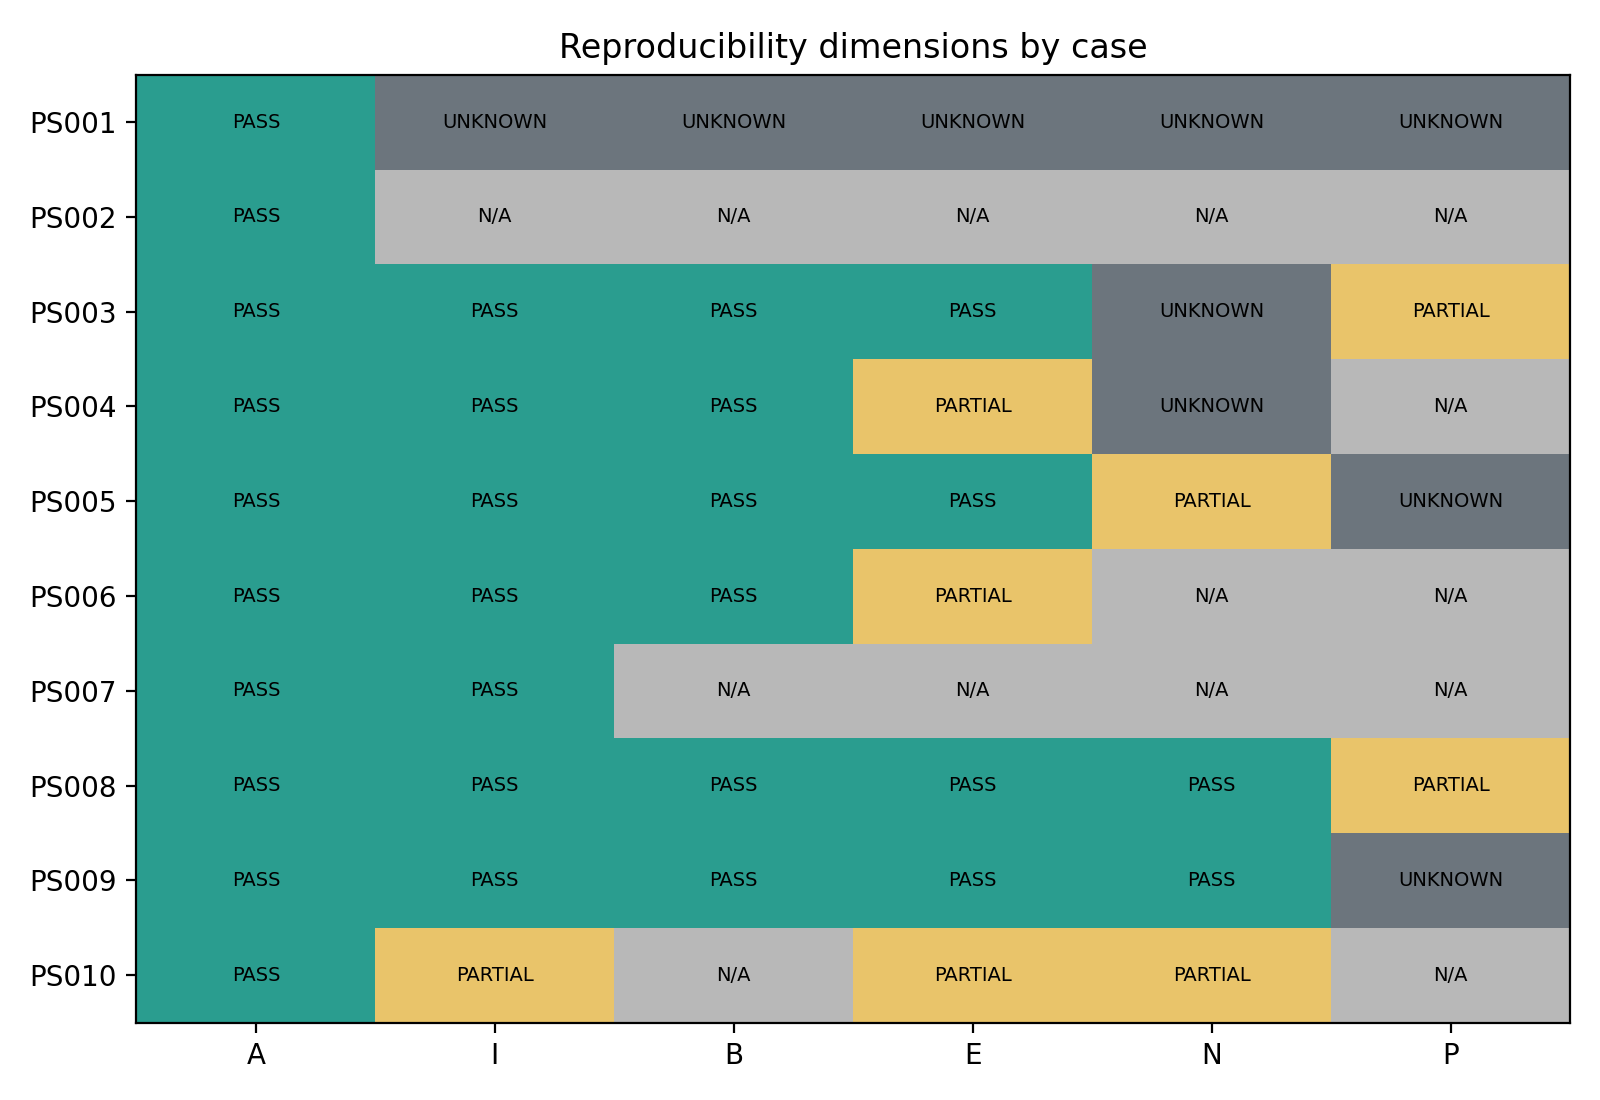
\includegraphics[width=0.92\textwidth]{Figure_03.png}
\caption{Long-term reproducibility status across the ten evaluated artifacts. Rows are cases PS001--PS010 and columns are the six capabilities A/I/B/E/N/P. N/A denotes an inapplicable or externally ineligible capability; UNKNOWN denotes insufficient retained evidence and is not counted as failure.}
\label{fig:3}
\end{figure*}

\subsection{Layered reproducibility outcomes}

All ten artifacts remained available. Installability was \texttt{PASS} for 7/8 eligible cases (87.5\%) and \texttt{PARTIAL} for 1/8 (12.5\%). Buildability was \texttt{PASS} for 6/6 eligible cases (100\%). Executability was \texttt{PASS} for 4/7 eligible cases (57.1\%) and \texttt{PARTIAL} for 3/7 (42.9\%). Numerical/scientific fidelity was \texttt{PASS} for 2/4 eligible cases (50.0\%) and \texttt{PARTIAL} for 2/4 (50.0\%). Performance fidelity was evaluated in only two eligible cases; both were \texttt{PARTIAL} (2/2), with no \texttt{PASS} case.

Availability and successful buildability did not imply downstream scientific or performance fidelity. Denominators contract at later layers because hardware constraints, non-applicable dimensions, and missing traces prevent legitimate classification.

The supplementary aggregate capability-profile figure retains the dimension-level distributions and excluded states. It is intentionally not interpreted as a case-level flow because eligibility changes by dimension; the adjacent-transition analysis in Section 5.1.2 remains the appropriate case-level evidence.



\begin{table*}[t]
\centering
\caption{Dimension-specific observed denominators. Percentages refer only to PASS/PARTIAL/FAIL cells; N/A and UNKNOWN are reported separately and excluded from the denominator.}
\label{tab:5}
\footnotesize
\setlength{\tabcolsep}{3pt}
\begin{tabularx}{\textwidth}{@{}>{\raggedright\arraybackslash}X>{\raggedright\arraybackslash}X>{\raggedright\arraybackslash}X>{\raggedright\arraybackslash}X>{\raggedright\arraybackslash}X>{\raggedright\arraybackslash}X>{\raggedright\arraybackslash}X@{}}
\toprule
Dimension & PASS & PARTIAL & FAIL & Eligible denominator & Excluded N/A & Excluded UNKNOWN \\
\midrule
A & 10 (100.0\%) & 0 & 0 & 10 & 0 & 0 \\
I & 7 (87.5\%) & 1 (12.5\%) & 0 & 8 & 1 & 1 \\
B & 6 (100.0\%) & 0 & 0 & 6 & 3 & 1 \\
E & 4 (57.1\%) & 3 (42.9\%) & 0 & 7 & 2 & 1 \\
N & 2 (50.0\%) & 2 (50.0\%) & 0 & 4 & 3 & 3 \\
P & 0 & 2 (100.0\%) & 0 & 2 & 5 & 3 \\
\bottomrule
\end{tabularx}
\\[2pt]
\footnotesize\emph{Note:} N (n=4) and P (n=2) are descriptive only. They are not interpreted as population rate estimates; no inferential claim is made for P.
\end{table*}

\subsubsection{Sensitivity to partial and unknown outcomes}

Counting only \texttt{PASS}, the observed rates for I, B, E, N, and P were 87.5\%, 100.0\%, 57.1\%, 50.0\%, and 0.0\%. Under an inclusive rule that counts \texttt{PASS} or \texttt{PARTIAL}, each observed eligible denominator reached 100\%. Treating applicable \texttt{UNKNOWN} cells as failures or successes produced the following strict-pass bounds: I 77.8--88.9\%, B 85.7--100.0\%, E 50.0--62.5\%, N 28.6--71.4\%, and P 0.0--60.0\%.

\textbf{Uncertainty.} These bounds are classification sensitivity analyses, not confidence intervals or population estimates. They expose the influence of unavailable traces without assigning those cells invented outcomes.

\begin{figure*}[t]
\centering
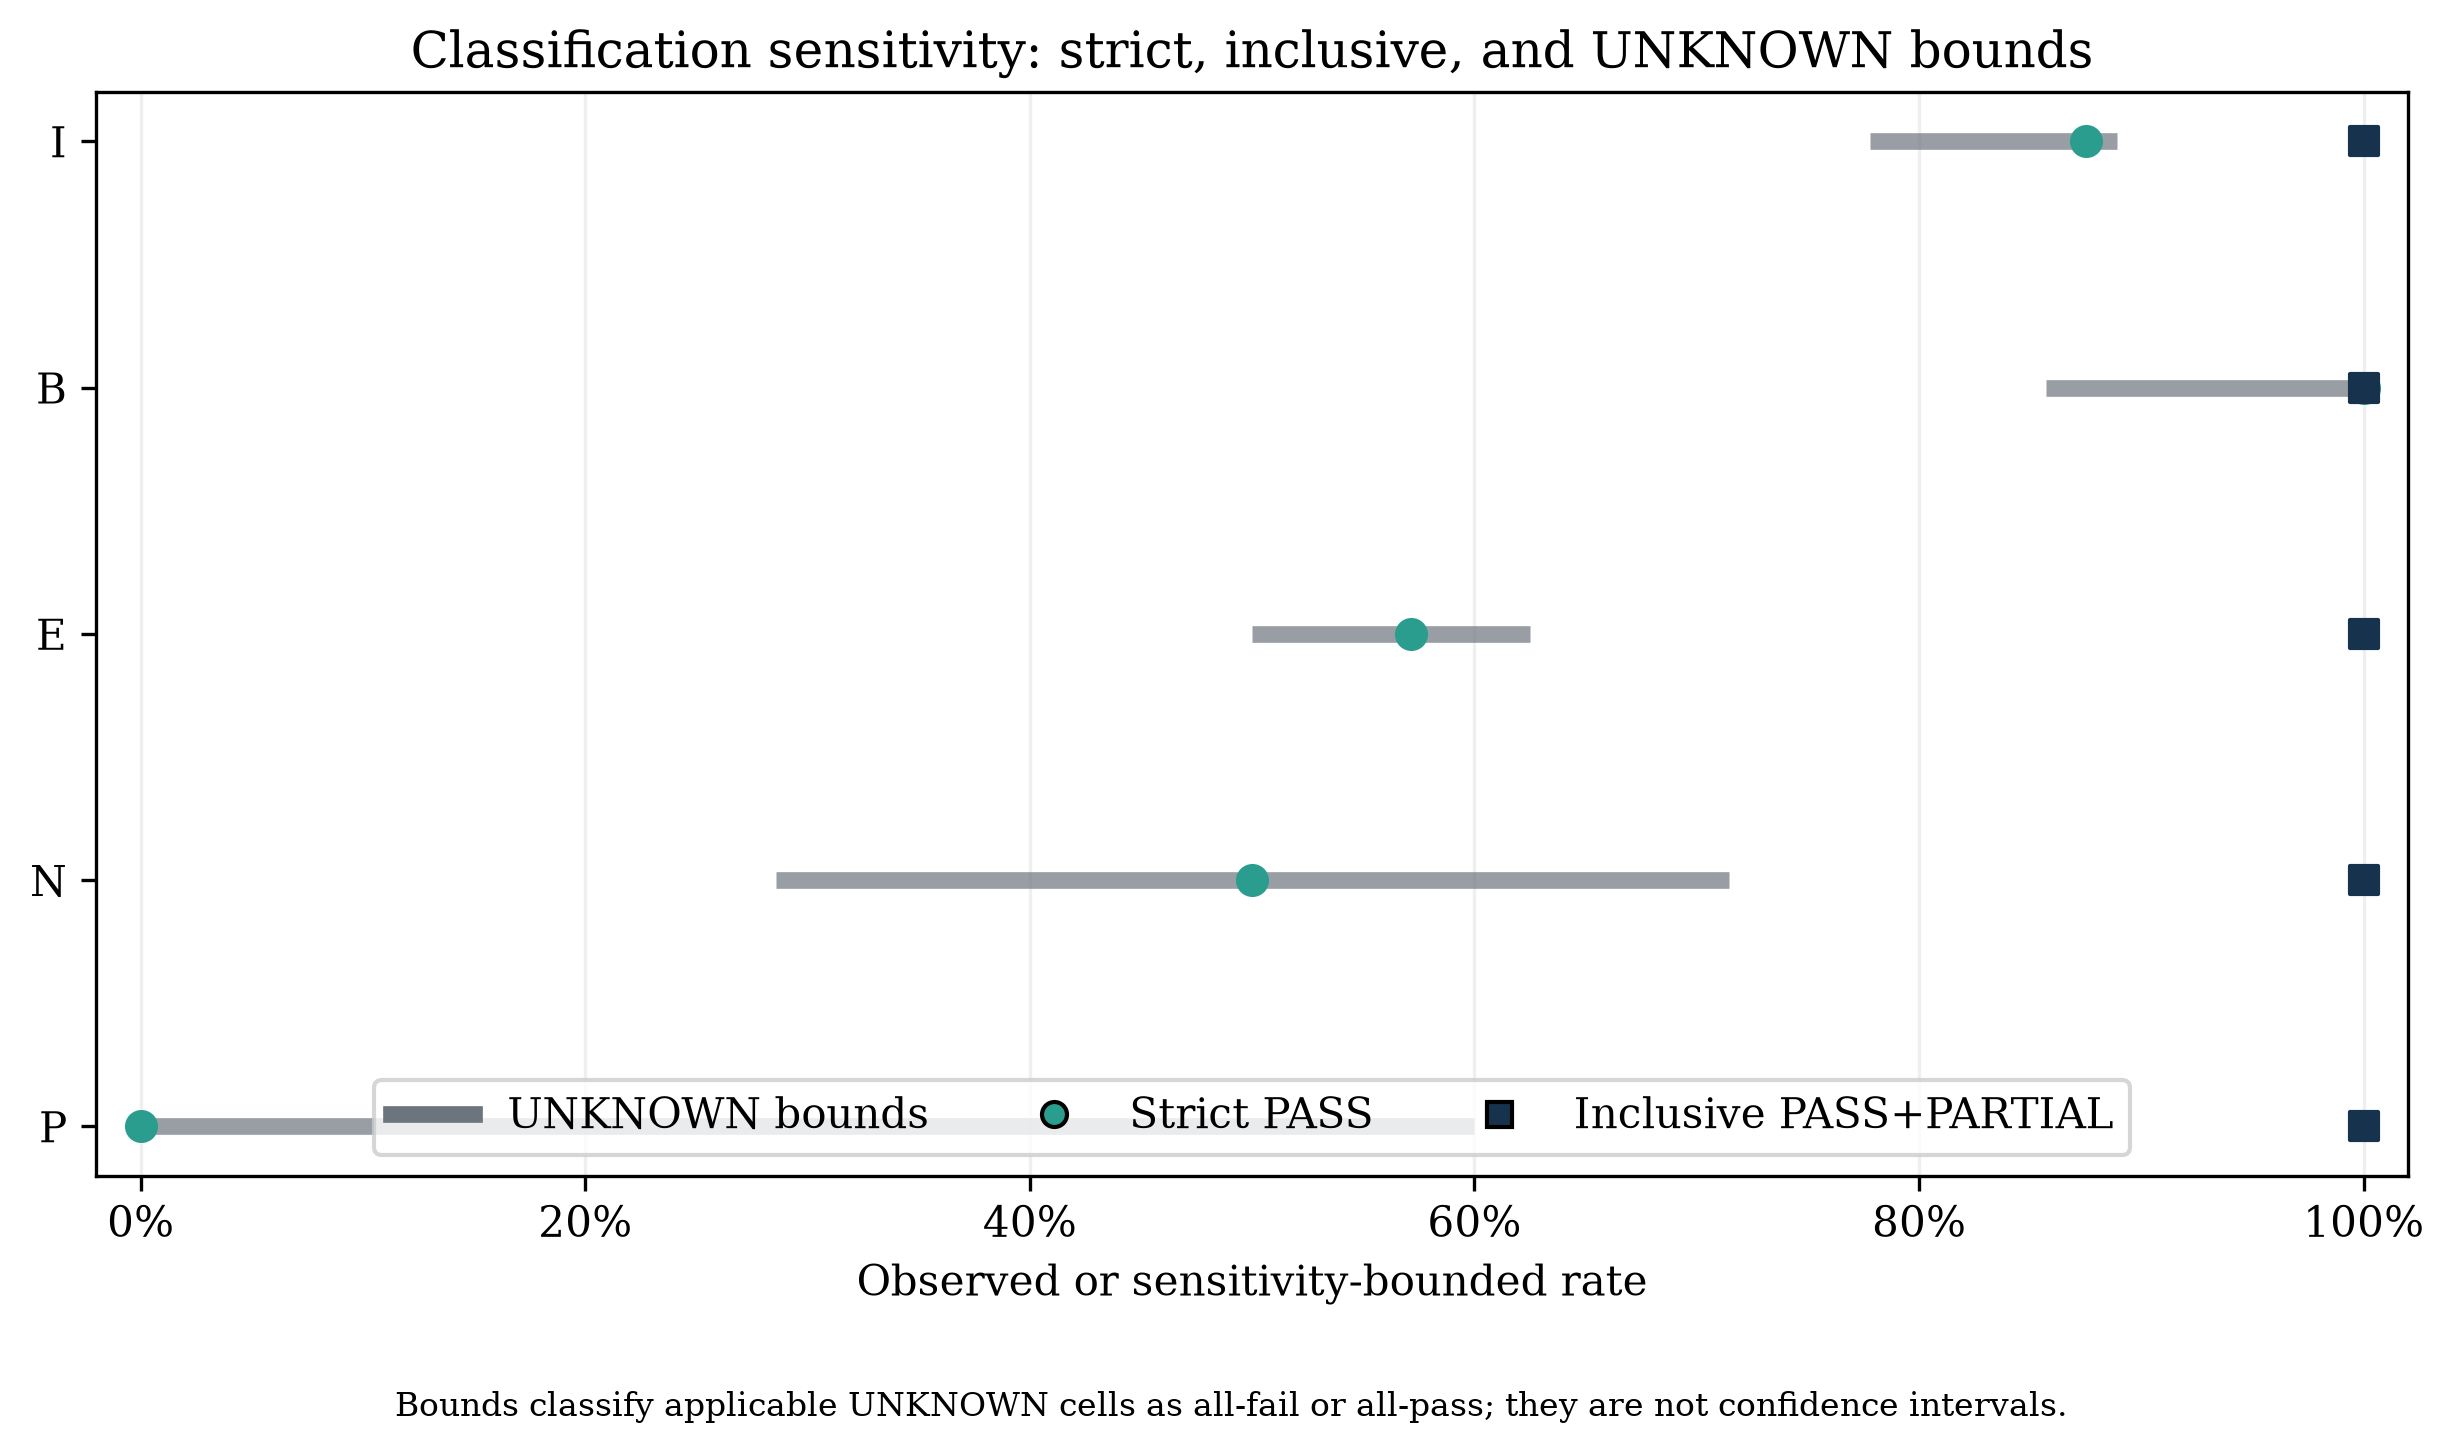
\includegraphics[width=0.92\textwidth]{Figure_04.png}
\caption{Classification sensitivity for installability, buildability, executability, scientific-result fidelity, and performance fidelity. Points show strict PASS and inclusive PASS-or-PARTIAL rates; horizontal ranges show worst/best reassignment of applicable UNKNOWN cases and are not confidence intervals.}
\label{fig:4}
\end{figure*}

The useful contrast is not between success and failure alone. Full \texttt{PASS} support became less common at later layers, while uncertainty widened as fewer cases remained classifiable.

\subsubsection{Observed chain breakpoints}

Across the ordered dimensions, five cases showed a directly comparable decrease: A-to-I for PS010, B-to-E for PS004 and PS006, E-to-N for PS005, and N-to-P for PS008. The remaining cases either showed no observed adjacent decrease or lacked comparable downstream states.

\textbf{Evidence and denominator.} Among cases with comparable adjacent states, degradation occurred in 1/8 for A-to-I, 0/6 for I-to-B, 2/6 for B-to-E, and 1/4 for E-to-N. The single comparable N-to-P case (PS008) showed a degradation from \texttt{PASS} to \texttt{PARTIAL}; with a single case, no transition rate can be estimated. These transition-specific denominators differ and must not be combined into a single prevalence estimate.

These breakpoints make the layered representation useful for this corpus, while the transition-specific denominators are too small to imply any universal ordering of failure probabilities.

\subsection{RQ1 — Long-term reproducibility}

Only one case executed successfully out of the box. Three cases that initially failed later reached execution \texttt{PASS} after repair, and three cases reached only partial execution. Two cases were excluded from execution because hardware or infrastructure prerequisites were unsatisfied, and one case remained unknown because its historical execution trace was unavailable.

Within this corpus, recovered execution was more common than out-of-the-box success. PS002 and PS007 demonstrate why an unsatisfied external prerequisite must be separated from software execution failure.

\begin{tcolorbox}[answerbox,title=\textbf{RQ1 answer in brief}]
Availability was universal in the closed corpus, but downstream capability was not. Only one case executed out of the box; three initially failing cases were recovered to execution \texttt{PASS}, three remained partial, two were externally ineligible, and one historical execution remained evidentially unknown. The result supports a layered rather than binary notion of long-term reproducibility.
\end{tcolorbox}

\begin{figure*}[t]
\centering
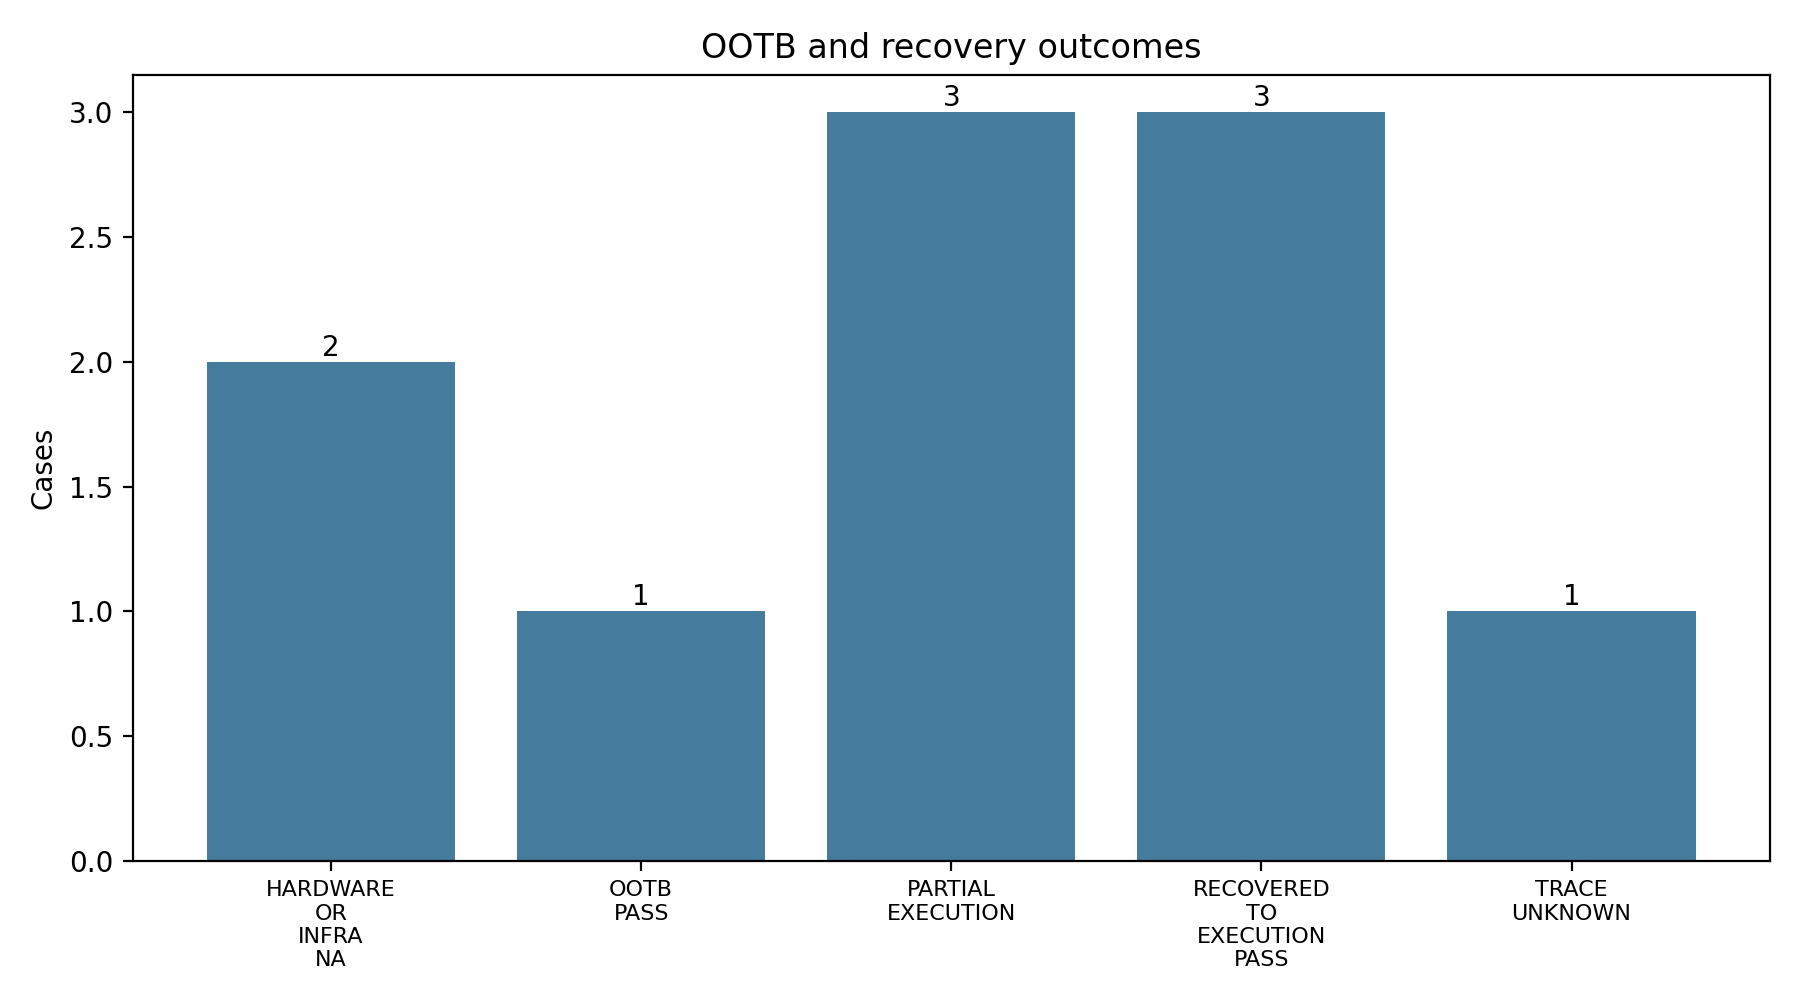
\includegraphics[width=0.92\textwidth]{Figure_05.png}
\caption{Execution outcome before and after bounded intervention. The figure separates out-of-the-box execution from eventual recovery and therefore does not treat an initial failure as irrecoverability.}
\label{fig:5}
\end{figure*}

\subsection{RQ2 — Failure mechanisms}

The observed mechanisms were heterogeneous. Dependency decay, toolchain drift, performance drift, and trace decay each occurred in two cases. Runtime version sensitivity (PS003), runtime semantic drift (PS010), environment/encoding coupling (PS004), hardware constraint (PS002), infrastructure constraint (PS007), and workflow/data-orchestration blockage (PS006) were each observed in one case. Mechanism counts are non-exclusive and therefore do not sum to ten. The broad \texttt{RUNTIME\_API\_DRIFT} label used during exploratory coding was retired because the retained evidence did not justify treating JDK sensitivity, Windows encoding behavior, dependency reconstruction, and R semantic incompatibility as one mechanism.

The observed impediments were distributed across dependency, runtime, toolchain, workflow, hardware, infrastructure, performance, and evidentiary layers rather than forming one uniform failure class.

\begin{tcolorbox}[answerbox,title=\textbf{RQ2 answer in brief}]
No single mechanism explains the observed degradation. Dependency decay, toolchain drift, runtime sensitivity or semantic drift, environment coupling, workflow blockage, external hardware/infrastructure constraints, performance drift, and trace decay occur at different layers and can co-occur in one case.
\end{tcolorbox}

\begin{figure*}[t]
\centering
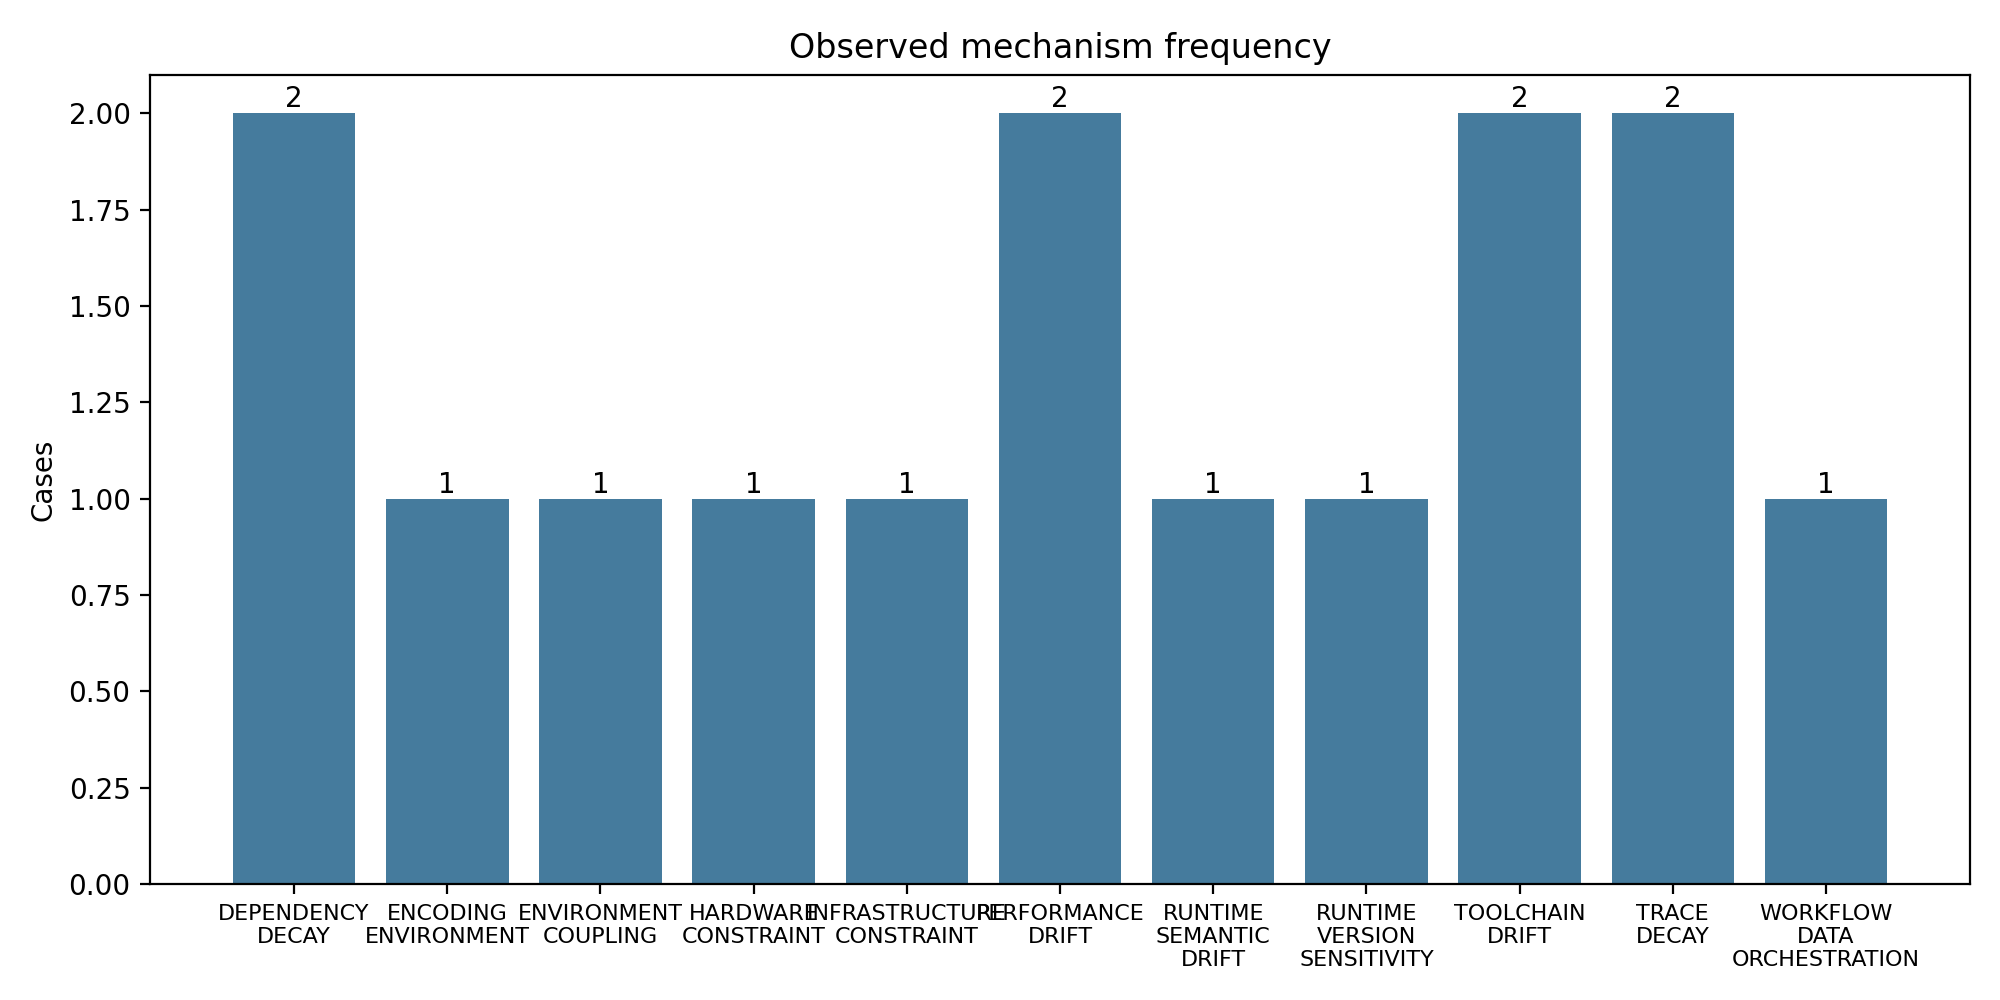
\includegraphics[width=0.92\textwidth]{Figure_06.png}
\caption{Non-exclusive technical mechanisms identified in the retained evidence. A case can contribute to more than one mechanism; mechanism frequency is therefore not an artifact-level failure rate.}
\label{fig:6}
\end{figure*}

\subsection{RQ3 — Repairability}

Repair depth also varied. Among cases with evidenced intervention depth, the final maximum repair levels were RL0 for four cases, RL2 for three, and RL3 for two; no case was classified RL1 or RL4. PS001 is recorded separately as \texttt{UNRECOVERED}/trace-incomplete rather than as a repair level. Three initially failing cases reached execution \texttt{PASS}; other repaired cases remained partial.

Recovery generally required dependency/toolchain or build/workflow intervention, but no retained case required a scientific source-code modification. PS001's unrecovered status describes trace loss for the historical experiment and is not an artifact-failure verdict.


\begin{tcolorbox}[answerbox,title=\textbf{RQ3 answer in brief}]
Bounded intervention recovered execution in several cases without changing scientific source logic, but repairability was not equivalent to full reproducibility. The maximum repair level records how far reconstruction had to depart from the original path, while unrecovered or trace-incomplete cases remain explicit rather than being forced into a success/failure binary.
\end{tcolorbox}

\subsection{RQ4 — Scientific-result and performance fidelity}
\subsubsection{Scientific-result fidelity}

Scientific-result evidence varied in strength across cases. PS008 retained zero checksum differences or explicit \texttt{PASSED} checksum results for selected kernels. PS009 retained \texttt{Verification = SUCCESSFUL} for EP and MG OpenMP C++ Class S and CG SER C++ Class S; these outputs are not treated as one homogeneous implementation. PS005 completed and reported aggregate precision 0.526, recall 0.688, and F1 0.556, but equivalence to the publication was only partially established. PS010 produced two PDFs before terminating in \texttt{mgmsampler}, so its scientific fidelity remained partial. PS001 supplied no recoverable historical MSE/MAE values.

Internal verification and checksum success provide stronger numerical evidence than successful process completion alone. In the decision rule used here, \texttt{N=PARTIAL} means that a scientifically meaningful subset of the declared output or validation target is retained, while full equivalence to the author-reported target is not established. This is why PS005 and PS010 remain partial rather than \texttt{PASS}; unavailable or non-comparable evidence remains \texttt{UNKNOWN} rather than being promoted from process completion alone.


\begin{table*}[t]
\centering
\caption{PS001 publication-level predicates and prohibited interpretations. All numerical entries come from the publication; none is an \texttt{OUR-OBSERVED} result.}
\label{tab:6}
\footnotesize
\setlength{\tabcolsep}{3pt}
\begin{tabularx}{\textwidth}{@{}>{\raggedright\arraybackslash}X>{\raggedright\arraybackslash}X>{\raggedright\arraybackslash}X>{\raggedright\arraybackslash}X>{\raggedright\arraybackslash}X@{}}
\toprule
Dataset / horizon & Compared methods & Displayed MSE & Supported paper-level predicate & Not supported \\
\midrule
Electricity / 96 & DLinear vs FEDformer & 0.140 vs 0.193 & \texttt{MSE(DLinear) < MSE(FEDformer)} & Reproduced value or local N=\texttt{PASS} \\
Electricity / 96 & DLinear vs Linear & 0.140 vs 0.140 & Tie at displayed precision & \texttt{MSE(DLinear) < MSE(Linear)} \\
Exchange-Rate / 96 & DLinear vs FEDformer & 0.081 vs 0.148 & \texttt{MSE(DLinear) < MSE(FEDformer)} & Reproduced value or causal explanation \\
Exchange-Rate / 96 & DLinear vs Repeat & 0.081 vs 0.081 & Tie at displayed precision & \texttt{MSE(DLinear) < MSE(Repeat)} \\
\bottomrule
\end{tabularx}
\end{table*}

\subsubsection{Performance fidelity}

For PS003, the baseline-adjusted mean \protect\path{ijOps/sjOps} ratios were 139.06 under Temurin 17, 79.47 under Temurin 21, and 61.06 under Temurin 25. Across three independent repetitions per JDK, coefficients of variation were 13.57\%, 50.53\%, and 34.46\%, respectively. The corresponding two-sided 95\% t intervals were wide, particularly for JDK 21; no inferential cross-JDK test was applied with only three independent repetitions per condition.

The two performance-eligible cases were both classified \texttt{PARTIAL}. Here \texttt{P=PARTIAL} means that performance was measured and scientifically interpretable, but full fidelity/comparability was not established: PS003 showed strong runtime sensitivity and substantial between-repetition variability, while PS008 compared confounded reconstructed configurations. The observed 2/2 configuration is therefore descriptive and does not constitute a performance-fidelity rate beyond these two cases.

PS003 performance was sensitive to the tested JDK configuration, but the retained data do not justify a monotonic causal effect of JDK version. The decrease in the mean baseline-adjusted ratio from 139.06 (JDK 17) to 79.47 (JDK 21) and 61.06 (JDK 25) is accompanied by substantial dispersion, especially under JDK 21 (CV=50.53\%). The wide descriptive intervals overlap across configurations, so the visual ordering in Fig.~\ref{fig:7} should be read as runtime sensitivity within the evaluated setup, not as evidence of a population-level version trend.

\par\medskip\noindent
\begin{minipage}{\columnwidth}
\centering
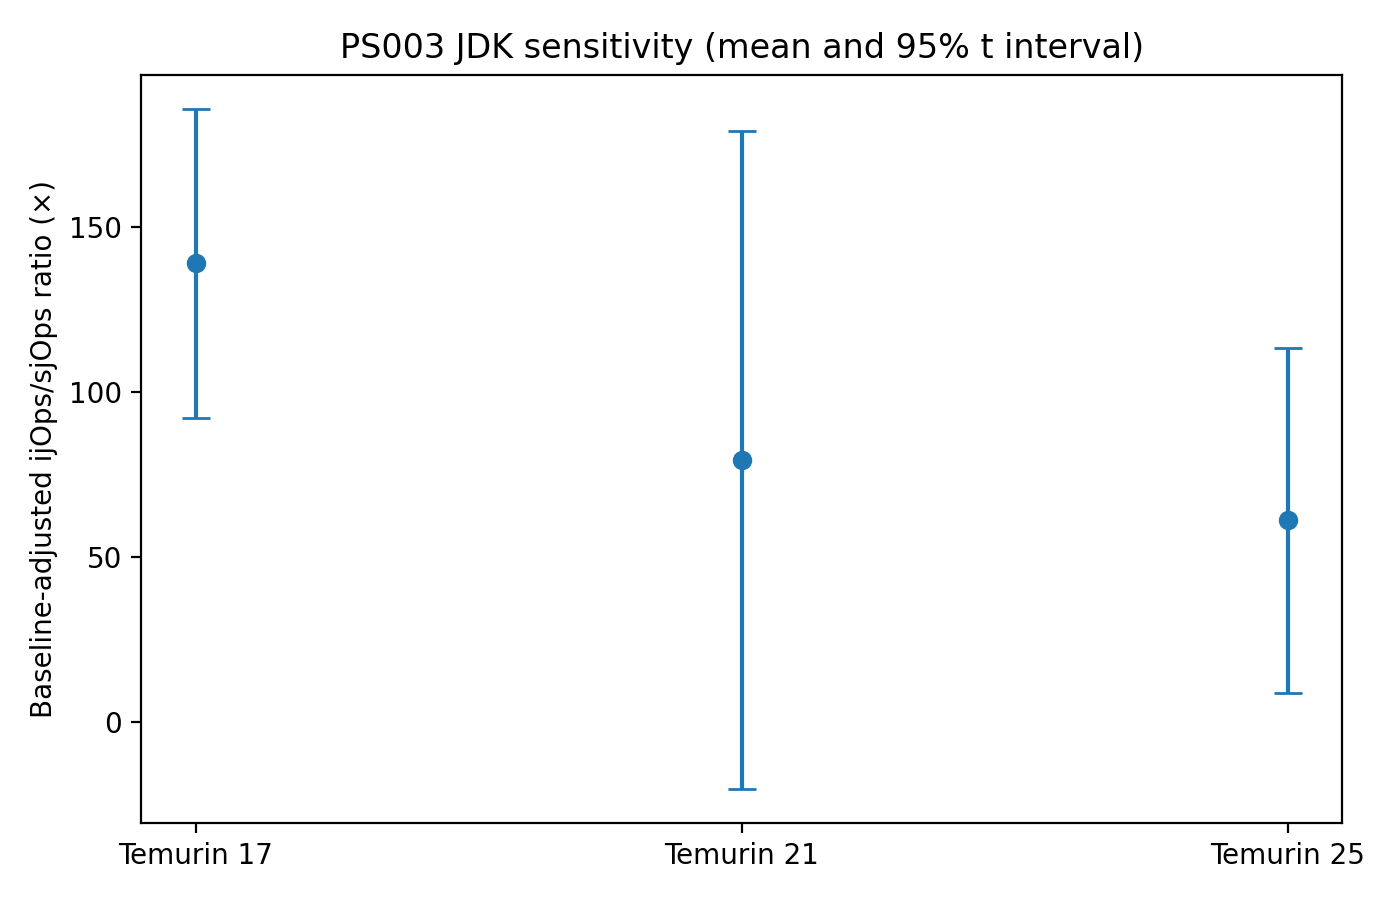
\includegraphics[width=0.96\columnwidth]{Figure_07.png}
\refstepcounter{figure}\label{fig:7}
\smallskip
{\small\textbf{Fig. \thefigure.} PS003 runtime sensitivity across JDK configurations. Points are baseline-adjusted mean ijOps/sjOps ratios and intervals are descriptive 95\% t intervals across three retained independent repetitions per JDK; no population-level JDK effect is inferred.\par}
\end{minipage}
\par\medskip

Fig.~\ref{fig:7} supports the \texttt{P=PARTIAL} classification for PS003. Performance remains measurable under each retained JDK, yet the combination of large between-configuration shifts and high within-configuration variability prevents a full fidelity claim. In other words, the experiment remains executable and benchmarkable, but its performance behavior is not stable enough to treat runtime as a preserved property across the evaluated runtime configurations.

For PS008, retained current/historical Base\_Seq mean runtimes were respectively 0.675188/2.010450 s for DAXPY, 1.662521/5.633594 s for TRIAD, and 0.100516/0.268251 s for REDUCE\_SUM. Both reconstructed configurations retained successful selected-kernel checksum evidence.

Performance values were not preserved across the two reconstructed PS008 configurations. The historical-to-current runtime ratios are approximately 2.98 for DAXPY, 3.39 for TRIAD, and 2.67 for REDUCE\_SUM. Because commits, submodules, compiler/build choices, and environmental factors differ, these ratios describe configuration-level differences and do not isolate software version as a causal factor.

\par\medskip\noindent
\begin{minipage}{\columnwidth}
\centering
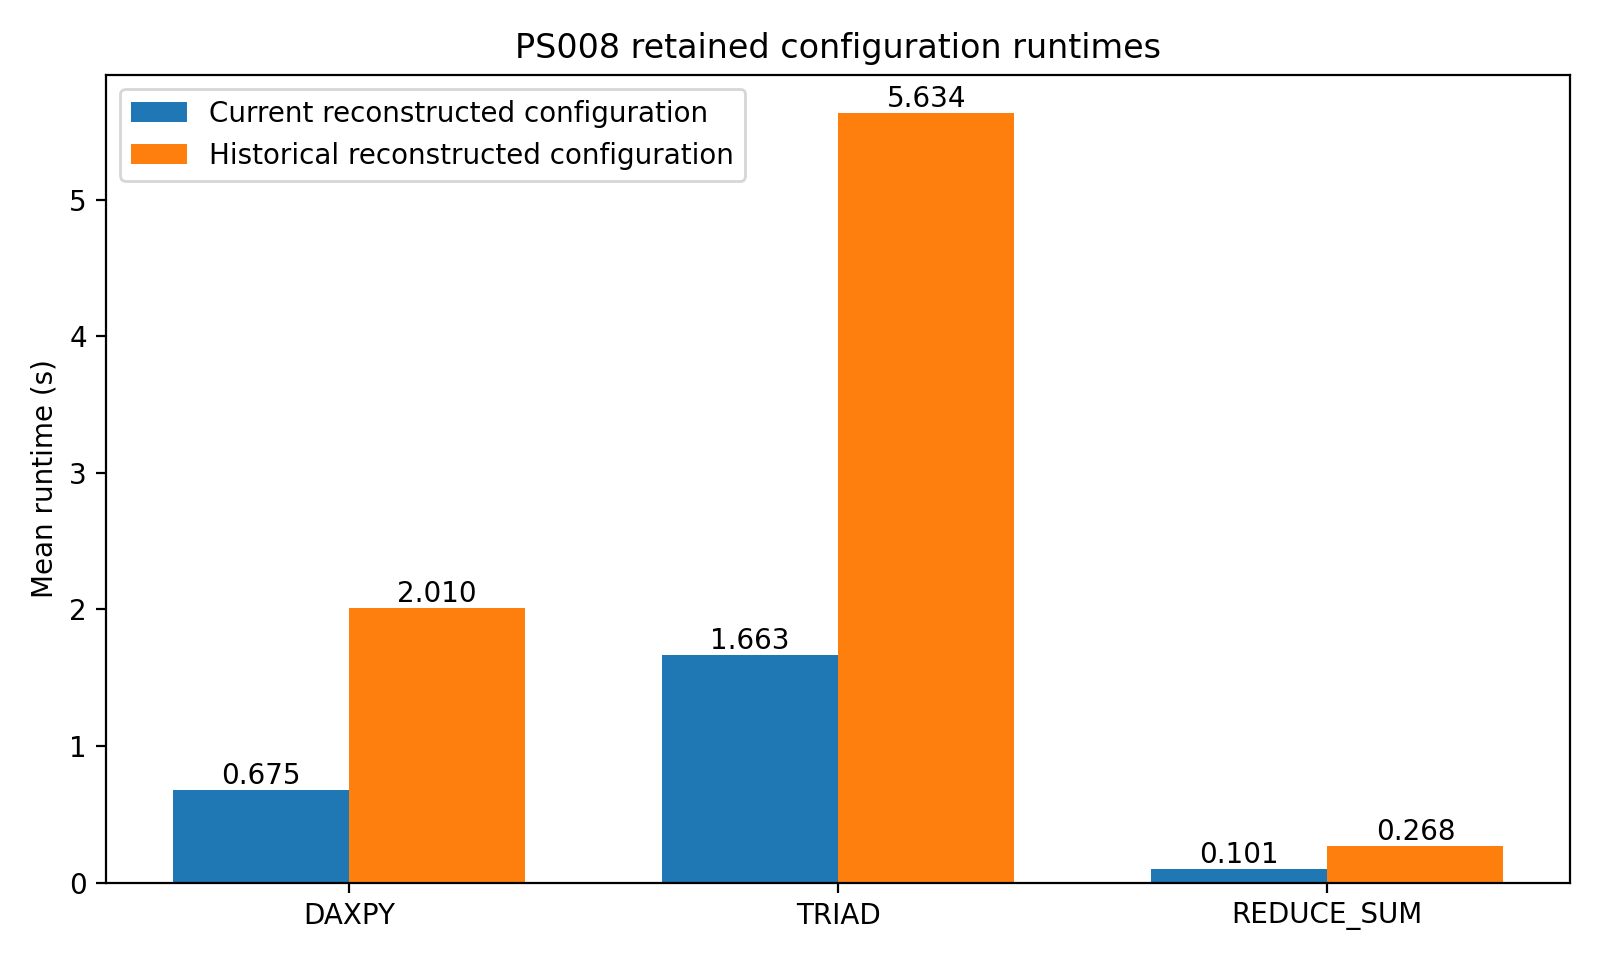
\includegraphics[width=0.96\columnwidth]{Figure_08.png}
\refstepcounter{figure}\label{fig:8}
\smallskip
{\small\textbf{Fig. \thefigure.} PS008 Base\_Seq runtimes for historical and current reconstructed configurations. The comparison is descriptive because code and environment differences are confounded; it must not be interpreted as a causal software-version effect.\par}
\end{minipage}
\par\medskip

Fig.~\ref{fig:8} provides the clearest within-corpus separation between scientific-result fidelity and performance fidelity. The selected kernels retained successful checksum evidence in both reconstructed configurations, while their measured runtimes differed markedly. The contrast supports treating N and P separately: a computation can remain numerically valid even when performance comparability is weakened. The figure does not establish that RAJAPerf itself became faster; it shows only that performance was not preserved across the two confounded reconstructed configurations.

\begin{tcolorbox}[answerbox,title=\textbf{RQ4 answer in brief}]
Execution, scientific-result fidelity, and performance fidelity were empirically separable. Artifact-native verification could remain valid while performance comparability weakened, most clearly in PS008. Accordingly, numerical correctness (N) cannot be used as a proxy for performance preservation (P), and successful execution alone establishes neither.
\end{tcolorbox}

\subsection{Preservation mechanisms and external prerequisites}

The preservation mechanisms exposed different external dependencies. PS002 supplied a CUDA container but required an unavailable NVIDIA GPU. PS007 supplied a VirtualBox VM because BenchExec was unsuitable for Docker, yet the retained host could not satisfy the infrastructure execution path. PS010 preserved source-level examples but not the complete historical R dependency ecosystem. PS005 benefited from a reconstructable pinned Python environment, while PS009 required build/workflow repair whose exact historical sequence remains trace-incomplete.

Containers, VMs, dependency specifications, and build metadata preserved different parts of the reproducibility chain; none independently guaranteed that hardware, infrastructure, ecosystem resolution, execution, and fidelity would all remain satisfiable.

A supplementary preservation-scope map formalizes this interpretation. Its cells encode what each packaging mechanism documents or leaves contingent in the retained examples; they are not additional case outcomes and do not alter the official matrix. In particular, a documented software environment does not preserve an external GPU or guarantee that a VM will start on a future host.

\section{Discussion}

\subsection{From artifact survival to capability survival}

Within this closed corpus, continued artifact availability did not determine how far downstream reproducibility remained supportable. All ten artifacts were available, yet the retained evidence diverged at dependency resolution, build and execution, scientific validation, performance comparison, external eligibility, and trace provenance. The model is therefore best interpreted as a \textbf{layered capability diagnostic}, not as a universal causal chain or a population model of failure probability.

This also sharpens the title question, \emph{what breaks?} Here, ``break'' denotes a loss, thinning, or non-evaluability of a capability or its evidentiary support---not necessarily a final \texttt{FAIL} cell. PS002 retained a CUDA-oriented container while the evaluated host lacked the required NVIDIA device; PS007 retained a VM-oriented path without a satisfiable infrastructure path; PS010 preserved source examples but not the complete historical R dependency ecosystem. Containers, VMs, dependency specifications, and build metadata therefore preserve different scopes of the chain rather than guaranteeing future reproduction \citep{boettiger2015docker,chan2023rang,guilloteau2024longevity}.

PS001 and PS009 additionally expose \textbf{trace decay}: software behavior and evidentiary continuity can age independently. During taxonomy refinement, the exploratory category \texttt{RUNTIME\_API\_DRIFT} also proved too coarse to be supported consistently by the retained evidence. We therefore use narrower mechanism labels---for example runtime version sensitivity for PS003, environment/encoding for PS004, dependency decay for PS005, and dependency decay plus runtime semantic drift for PS010---and claim concrete API drift only when an incompatibility is directly evidenced.

\subsection{Recoverability changes the meaning of failure}

Three initial failures reached execution \texttt{PASS} after bounded intervention. The evidenced repairs were concentrated at RL2 and RL3, and no retained case required RL4 scientific source-code modification. A binary evaluation performed only at the first failed command would therefore have conflated immediate reproducibility with irrecoverability. The distinction matters for software evolution: dependency/toolchain and build/workflow repairs can restore downstream capability without changing the scientific algorithm.

Repair level is not a severity score and is no longer used to encode an unrecovered outcome. Intervention depth (RL0--RL4), capability state (A/I/B/E/N/P), recovery status, and mechanism answer different questions: \emph{how much was changed}, \emph{what ultimately worked}, \emph{whether recovery succeeded}, and \emph{why the path was impeded}. Keeping these axes separate is necessary for interpretable longitudinal artifact evaluation.

\subsection{Correctness and performance age differently}

PS008 and PS009 retained benchmark-native correctness evidence through checksums or verification. PS008 nevertheless exhibited substantially different timings across confounded reconstructed configurations. PS003 provided a controlled runtime-sensitivity experiment in which performance ratios and between-repetition variability differed across tested JDKs, while no independent scientific-correctness oracle was retained for N. These cases justify the operational separation \(E\neq N\neq P\).

\texttt{N=PASS} means that a declared artifact-specific scientific criterion was satisfied within scope; it does not imply performance preservation. Conversely, \texttt{P=PARTIAL} does not mean that performance ``failed'': it means performance evidence was available and interpretable but full comparability could not be established because of runtime sensitivity, variability, or documented confounding. With only four N-eligible and two P-eligible cases, these observations are diagnostic rather than rate estimates.

\subsection{Implications for artifact engineering and evaluation}

The cross-case evidence suggests that durable artifacts should preserve a \textbf{claim-to-evidence path}, not only source code. Exact source revisions and input checksums should be accompanied by machine-readable runtime, compiler, system-library and dependency information; build and execution commands; raw stdout/stderr and generated outputs; explicit hardware/infrastructure prerequisites; artifact-native correctness oracles; and performance protocols that are preserved separately from correctness checks. Containers and VMs remain valuable, but their host, driver, device, and hypervisor assumptions should be explicit and persistently identified.

For artifact evaluators, layered states and explicit \protect\path{N/A}/\texttt{UNKNOWN} values prevent missing hardware, trace loss, partial execution, and scientific failure from being collapsed into one label. Reporting both initial and recovered states distinguishes immediate reproducibility from recoverability. These implications are grounded in the observed mechanisms of this corpus; they are not population-wide estimates.

The evidence does not support stronger population-level claims. The ten purposively selected cases cannot estimate prevalence across scientific software; PS008 cannot support a causal software-version effect because reconstructed configurations are confounded; and repository-level quality practices cannot be linked causally to scientific stability from this matrix. Future work should use independently sampled paper--repository pairs, preregistered claim oracles and tolerances, controlled environment perturbations, repeated runs, and independent human coding.

\section{Threats to Validity}

\subsection{Construct validity and coding reliability}

Layer definitions and \texttt{PASS}/\texttt{PARTIAL}/\texttt{FAIL} decisions depend on operational rules. Safeguards include a controlled vocabulary, explicit dimension definitions, case-level evidence reports, benchmark-native validation where available, a 47-row claim-to-evidence appendix, and a versioned coding/adjudication record. No independent blinded second-coder exercise was conducted; consequently, no inter-rater reliability coefficient is reported, and the classifications should be read as team-adjudicated judgments.

\subsection{Internal validity and evidence completeness}

Repairs may alter behavior. Every evidenced intervention is assigned RL0--RL4, with environmental/build repairs separated from scientific source changes; no retained case is classified RL4. Recovery status is recorded independently. Some historical before/after chains remain incomplete, particularly PS004 and PS009, so causal repair-mechanism claims are avoided. Historical PS001 MSE/MAE and environment traces were not recovered, and standalone host/VM traces are absent for PS002 and PS007. Missing evidence is represented as \texttt{UNKNOWN}, \texttt{NOT\_FOUND}, or trace-incomplete rather than reconstructed. Fresh executions can strengthen contemporary observations but cannot retroactively restore historical provenance.

\subsection{External validity}

The ten purposively selected heterogeneous artifacts form a closed maximum-variation multiple-case corpus, not a random sample. Percentages characterize only this corpus and always include their eligible denominator. The approximately 180 person-hours invested in deep reconstruction provide context for this design choice but do not make the corpus statistically representative. The results support analytical transfer of the layered diagnostic proposition, not prevalence estimates for scientific software generally. This limitation cannot be removed by statistical treatment; it would require a separately designed larger sampling study. The design instead targets evidence that broader studies generally do not combine at case level: claim-level provenance, external eligibility, separated numerical/performance fidelity, and bounded repair histories \citep{runeson2009guidelines,muttakin2026openscience}.

\subsection{Statistical conclusion validity}

Late-stage denominators are small: four eligible cases for N and two for P. PS003 contains three independent repetitions per JDK, producing wide t intervals, especially for JDK 21; no underpowered inferential cross-JDK test is reported. PS008 configurations differ in code and environment, so timing differences are descriptive and non-causal. Sensitivity bounds expose rather than conceal the influence of \texttt{UNKNOWN} classifications. Mechanism counts are likewise descriptive and non-exclusive; no ecosystem-level significance test is attempted.

\section{Conclusion}

This study evaluated ten heterogeneous scientific-software artifacts with a layered capability model covering availability, installability, buildability, executability, numerical/scientific fidelity, and performance fidelity, while treating hardware/infrastructure satisfiability as an external eligibility condition. All ten artifacts remained available, yet downstream support became progressively thinner and more uncertain. Several initially failing artifacts were recoverable through bounded dependency/toolchain or build/workflow intervention without retained evidence of scientific source-code modification.

The central conclusion is diagnostic rather than prevalence-based: \textbf{artifact survival does not determine which scientific capability survives with it}. Out-of-the-box failure was not equivalent to irrecoverability; successful execution was not equivalent to full scientific fidelity; and numerical correctness did not establish performance fidelity. Containers, VMs, dependency specifications, and build metadata each preserved useful layers, but none guaranteed the continued satisfiability of hardware, infrastructure, ecosystem resolution, correctness evidence, performance protocols, and historical trace provenance.

These findings remain bounded by the purposive n=10 corpus, small late-stage denominators, missing historical traces, confounded performance comparisons, and the absence of an independent blinded second-coder reliability study. The approximately 180 person-hours invested in the ten reconstructions underscore that this design targets diagnostic depth rather than prevalence. The resulting practical recommendation is to preserve not only code, but the \textbf{claim-to-evidence path}—environment, commands, raw outputs, repair history, scientific oracle, performance protocol, and external prerequisites—needed to determine what remains reproducible years later.


\section*{Data and Code Availability}
A blinded replication package accompanies the manuscript during peer review. It contains the closed artifact inventory, execution metadata, retained raw logs and outputs, cryptographic evidence hashes, intervention records, claim-level provenance registry, normalized datasets, validation scripts, statistical-analysis code, and figure-generation scripts. A persistent public archive of this package will be cited and linked in the final version. The package distinguishes author-reported values from our observations and preserves \texttt{UNKNOWN} and \protect\path{N/A} states rather than reconstructing missing evidence.

\section*{Declaration of Competing Interest}
The authors declare that they have no known competing financial interests or personal relationships that could have appeared to influence the work reported in this paper.

\section*{Funding}
This research received no external funding.

\bibliographystyle{cas-model2-names}
\bibliography{references}
\end{document}
